% ============================================================
%  SimAeroMoE: Similarity-Aware Expert Deployment and Scheduling
%            for UAV Edge Inference
%  IEEE Transactions / Conference Format (IEEEtran)
% ============================================================

\documentclass[conference]{IEEEtran}

% ---- packages ------------------------------------------------
\usepackage[T1]{fontenc}
\usepackage[utf8]{inputenc}
\usepackage{cite}
\usepackage{amsmath,amssymb,amsfonts}
\usepackage{algorithmic}
\usepackage{algorithm}
\usepackage{graphicx}
\usepackage{cuted}
\usepackage{capt-of}
\usepackage{textcomp}
\usepackage{xcolor}
\usepackage{booktabs}
\usepackage{url}
\usepackage{array}
\usepackage{multirow}
\usepackage{tikz}
\usetikzlibrary{arrows.meta,positioning}
\usepackage{CJKutf8}

% 2. PDF注释支持
\usepackage{pdfcomment}
% 3. 确保注释使用Unicode编码
\hypersetup{unicode,hidelinks}

% circled number command (used for step annotations)
\newcommand{\circled}[1]{%
  \tikz[baseline=(char.base)]{%
    \node[shape=circle,draw,inner sep=1pt,font=\scriptsize] (char) {#1};}}

% keep long URLs from overflowing
\Urlmuskip=0mu plus 1mu

% compact float spacing for IEEE-style top-of-column figures
\setlength{\textfloatsep}{8pt plus 2pt minus 2pt}
\setlength{\floatsep}{8pt plus 2pt minus 2pt}
\setlength{\intextsep}{8pt plus 2pt minus 2pt}

% 允许更多置顶浮动体，避免图片堆积到文末
\setcounter{topnumber}{3}
\setcounter{dbltopnumber}{3}
\renewcommand{\topfraction}{0.90}
\renewcommand{\dbltopfraction}{0.90}
\renewcommand{\floatpagefraction}{0.70}
\raggedbottom

% ---- hyphenation hints ---------------------------------------
\hyphenation{op-tical net-works semi-conduc-tor Mix-ture-of-Ex-perts}

% ==============================================================
\begin{document}
\begin{CJK*}{UTF8}{gbsn}
\bstctlcite{IEEEexample:BSTcontrol}

% ---- title & authors -----------------------------------------
\title{SimAeroMoE: Similarity-Aware Expert Deployment and Scheduling
       for UAV Edge Inference}

\author{%
  \IEEEauthorblockN{%
    Liang Wei\IEEEauthorrefmark{1},
    Jiahao Lin\IEEEauthorrefmark{1},
    Ruoyu Tang\IEEEauthorrefmark{1},
    Xian Chen\IEEEauthorrefmark{2},
    and Hao Zhang\IEEEauthorrefmark{1}}
  \IEEEauthorblockA{\IEEEauthorrefmark{1}%
    School of Computer Science and Engineering,
    Southern Tech University, Guangzhou, China\\
    \{weiliang, linjiahao, tangruoyu, zhanghao\}@stu.edu.cn}
  \IEEEauthorblockA{\IEEEauthorrefmark{2}%
    Department of Electrical and Computer Engineering,
    University of Technology, Hong Kong SAR, China\\
    xian.chen@ust-ece.hk}
}

\maketitle

% ---- abstract ------------------------------------------------
\begin{abstract}
混合专家模型（Mixture-of-Experts, MoE）通过为不同任务激活部分专家，
为资源受限环境下的高效推理提供了一种可行思路。然而，在 UAV 边缘网络中
部署 MoE 模型仍面临多重挑战：UAV 的内存和计算能力有限，UAV 之间的
单跳通信链路带宽受限，不同任务对专家的需求分布也具有明显差异。若直接
部署所有原始专家，容易超过 UAV 的存储能力；若仅依据专家需求进行部署，
则可能忽略专家之间的相似替代关系以及跨 UAV 通信代价。

为解决上述问题，本文提出 SimAeroMoE，一种面向 UAV 边缘推理的相似性
感知专家部署与调度方法。SimAeroMoE 首先根据专家相似度构造可替代专家
集合，并将原始专家需求扩展为候选专家的有效需求；随后设计通信感知部署
评分，综合考虑专家需求、UAV 连通性、链路速率、计算能力和冗余部署成本。
在此基础上，SimAeroMoE 采用两阶段动态贪心部署策略：预部署阶段优先保证
必要专家需求可服务，动态调整阶段在 UAV 内存约束下进一步选择收益较高且
冗余较低的专家部署方案。最后，SimAeroMoE 基于部署结果进行轻量级逐层
推理调度，为每个专家执行步骤选择本地或单跳可达的 UAV。

仿真实验结果表明，在随机热点 UAV 场景下，SimAeroMoE 相比 Random
Placement、Importance 和 No-Sim 分别
降低了约 $24.1\%$、$21.3\%$ 和 $48.2\%$ 的平均端到端推理延迟。结果说明，
相似专家替代能够缓解 UAV 内存受限下的专家覆盖压力，通信感知部署能够
减少不必要的跨 UAV 传输，从而提升资源受限 UAV 边缘网络中的 MoE 协同
推理效率。
\end{abstract}

\begin{IEEEkeywords}
UAV edge computing, Mixture-of-Experts, expert deployment,
similarity-aware substitution, collaborative inference.
\end{IEEEkeywords}

\IEEEpeerreviewmaketitle

% ==============================================================
\section{Introduction}
\label{sec:intro}
% ==============================================================

随着边缘智能的发展，UAV 边缘网络逐渐成为低时延任务处理的重要平台。
UAV 可以根据任务区域灵活部署，并通过空中链路为地面用户提供计算与通信
服务，适用于应急感知、空中巡检、目标识别和协同监测等场景
~\cite{mozaffari2019uav,zhu2019uav}。与此同时，混合专家模型
（Mixture-of-Experts, MoE）通过稀疏激活机制仅调用部分专家完成推理，
在扩展模型容量的同时降低单次计算开销，因而为资源受限边缘环境中的智能
推理提供了新的可能~\cite{shazeer2017moe,fedus2022switch,jiang2024mixtral}。

然而，将 MoE 推理直接部署到 UAV 边缘网络中并不简单。首先，UAV 搭载的
计算和存储资源有限，难以在每个 UAV 上部署完整专家集合；当专家数量或专家
参数规模增加时，内存约束会成为主要瓶颈。其次，UAV 服务区域内的任务需求
具有明显的空间差异，不同区域可能频繁请求不同专家，简单的全局静态部署
难以适应这种区域化需求。最后，UAV 之间的无线链路带宽有限，本文考虑的
协同推理仅允许本地或单跳可达 UAV 参与专家执行；如果专家部署位置与任务
访问位置不匹配，中间特征需要频繁跨 UAV 传输，从而显著增加端到端延迟。

本文的关键观察是：MoE 专家之间并非完全独立，部分专家在参数或功能上具有
相似性。在 UAV 内存受限的情况下，如果某个原始所需专家无法直接部署，
可以在相似度满足阈值约束时使用可替代专家提供近似服务。该观察为专家部署
提供了额外弹性，但也带来新的设计问题：哪些专家可以作为替代候选，替代
需求如何计入部署收益，候选专家应部署在哪些 UAV 上，以及如何避免多个
相似专家在有限内存中造成冗余占用。

为解决上述问题，本文提出 \textbf{SimAeroMoE}，一种面向 UAV 边缘 MoE
推理的相似性感知专家部署与调度方法。SimAeroMoE 首先根据任务接入位置
统计各 UAV 区域的原始专家需求，并基于专家相似度构造可替代专家集合，
将原始需求扩展为候选专家的有效需求。随后，SimAeroMoE 设计通信感知的
部署评分，综合考虑专家需求、UAV 连通性、链路速率、计算能力以及冗余
部署成本。在此基础上，系统采用两阶段动态贪心部署策略：预部署阶段优先
保证必要专家需求可服务，动态调整阶段在剩余内存中选择收益更高且冗余更低
的专家部署方案。最后，SimAeroMoE 根据部署结果执行轻量级逐层推理调度，
为每个专家执行步骤选择本地或单跳可达的 UAV。

本文在随机热点 UAV 场景下对 SimAeroMoE 进行仿真实验，并与随机部署、
重要性优先部署和不考虑相似替代的部署方法进行比较。实验结果表明，
SimAeroMoE 相比 Random Placement、Importance 和
No-Sim 分别降低了约 $24.1\%$、$21.3\%$ 和 $48.2\%$
的平均端到端推理延迟，验证了相似专家替代、通信感知部署和动态贪心策略
在 UAV 边缘 MoE 协同推理中的有效性。

本文的主要贡献总结如下：
\begin{itemize}
  \item 建立 UAV 边缘网络中的 MoE 专家级协同推理模型，联合考虑 UAV
    计算能力、内存约束、单跳通信链路和任务专家序列对端到端延迟的影响。
  \item 提出相似性感知的候选专家构造方法和有效需求建模方法，将专家相似
    替代关系纳入 UAV 内存受限场景下的部署决策。
  \item 设计通信感知专家部署评分、两阶段动态贪心部署算法和轻量级逐层
    推理调度方法，并通过仿真实验验证其相对于多种基线方法的性能优势。
\end{itemize}

% ==============================================================
\section{Background and Motivation}
\label{sec:background}
% ==============================================================

\subsection{MoE Expert Inference}
\label{sec:bg_moe}

MoE 模型通过多个专家网络共同扩展模型容量，并由路由器或门控网络为
不同输入选择部分专家参与计算~\cite{shazeer2017moe,fedus2022switch,
lepikhin2021gshard,jiang2024mixtral}。与普通稠密模型相比，MoE 的核心
特点是\emph{稀疏激活}：一次推理并不需要调用所有专家，而是只执行与当前
任务相关的一小部分专家。因此，从计算角度看，MoE 可以在保持较大参数容量
的同时控制单次推理开销。

在本文考虑的任务级推理中，一个任务可以被表示为按顺序执行的专家序列。
例如，任务 $k$ 的第 $l$ 个推理步骤需要原始专家 $e_{k,l}$。如果该专家
已经部署在某个可访问 UAV 上，则该步骤可以在该 UAV 上执行；如果相邻步骤
由不同 UAV 执行，则需要在 UAV 之间传输中间特征。由此可见，MoE 推理在
边缘网络中的性能不仅取决于专家计算量，也取决于专家部署位置和跨节点通信
代价。

稀疏激活降低了单次计算需求，但并不自动消除部署压力。为了服务不同任务，
系统仍需要在边缘节点上保存若干专家参数。对于内存受限的 UAV 而言，关键
问题不再是是否执行整个模型，而是\emph{哪些专家应部署在哪些 UAV 上}。
该问题正是后续系统模型和方法设计关注的核心。

\subsection{Expert Deployment Challenges in UAV Edge Networks}
\label{sec:bg_uav_challenge}

UAV 边缘网络为 MoE 协同推理提供了灵活的空中计算平台，但也带来了比固定
边缘服务器更强的资源和通信约束。首先，每个 UAV 的可用内存有限，无法
简单部署全部专家。当专家数量增加，或某些专家参数规模较大时，全量部署会
迅速耗尽 UAV 存储资源，导致部分任务所需专家无法被服务。

其次，UAV 服务的地面任务通常具有空间热点特征。不同区域的用户、传感器或
应急目标可能产生不同类型的推理请求，从而导致不同 UAV 区域对专家的需求
分布并不相同。若所有 UAV 按相同方式静态部署专家，会浪费有限内存；若仅
按照全局专家重要性部署，又可能忽略局部高频任务需求。

第三，UAV-UAV 通信链路带宽受限且连通关系受空间位置影响。本文关注单跳
可达的协同推理场景：当某个任务的连续专家步骤分布在不同 UAV 上时，系统
需要通过单跳空空链路传输中间特征。如果高需求专家部署在距离任务接入 UAV
较远或不可达的位置，即使专家本身已经部署，也可能因为通信代价过高而增加
端到端延迟。因此，专家部署必须同时考虑任务需求、UAV 内存、计算能力以及
通信拓扑。

\subsection{Motivation for Similarity-Aware Deployment}
\label{sec:bg_similarity_motivation}

传统专家部署通常假设任务请求的原始专家必须由该专家本身执行。在内存充足
的云端或数据中心环境中，这一假设较为自然；但在 UAV 边缘网络中，这种
严格部署方式可能使系统陷入两难：若部署所有原始专家，UAV 内存不足；若
只部署少量高频专家，低频但必要的专家需求又可能无法覆盖。

本文利用的关键机会是专家之间的相似性。若专家 $e$ 与原始所需专家 $r$
在参数或功能表示上足够相似，则 $e$ 可以在相似度阈值约束下作为 $r$ 的
可替代专家。这样，系统不必机械地为每个原始专家保留独立部署空间，而可以
通过少量相似专家覆盖多个相近需求。例如，当某一区域频繁请求一个内存占用
较大的专家，而另一个轻量专家与其高度相似时，部署轻量替代专家可能更适合
内存受限的 UAV。

但是，相似替代不能单独决定部署方案。一个替代专家即使相似度较高，如果被
部署在通信不可达或链路速率较低的 UAV 上，也可能导致较大的中间特征传输
延迟；多个相似专家同时部署在相近位置，也可能造成冗余内存占用。因此，
相似性感知部署需要联合回答三个问题：哪些专家可以进入候选集合，替代后的
有效需求如何计算，以及候选专家应部署在哪些 UAV 上。上述动机直接引出
本文后续提出的 SimAeroMoE 设计：通过相似候选构造扩展可部署空间，通过
通信感知评分选择合适部署位置，并通过动态贪心策略在覆盖需求和控制冗余
之间取得平衡。


\section{System Model}
\label{sec:system}

本节建立一个准静态 UAV 边缘网络下的通用协同推理模型。
与传统 UAV 轨迹优化问题不同，本文不研究 UAV 在任务执行过程中的
飞行轨迹规划，而是假设在一个短时间调度窗口内，UAV 的空间位置
保持近似不变。因此，UAV 之间的无线拓扑、链路质量和可用通信容量
可以由当前空间位置和信道状态决定。基于该准静态网络，系统需要
决定任务由哪个 UAV 接入、哪些 UAV 参与协同推理、以及中间特征
如何在 UAV 网络中传输，从而最小化端到端推理延迟。
Fig.~\ref{fig:system_model} 展示了本文考虑的准静态 UAV 协同推理场景。

\begin{figure}[!t]
  \centering
  
\includegraphics[width=\columnwidth]{photo/system_model_uav_scenario.png}
  \caption{准静态 UAV 边缘网络中的协同推理场景。地面任务通过空地链路接入 UAV，多个资源异构 UAV 在给定无线拓扑下协同执行 MoE 推理计算单元，并通过 UAV-UAV 链路传输中间特征，最终将推理结果返回至基站或应急指挥中心。}
  \label{fig:system_model}
\end{figure}

\subsection{准静态 UAV 网络}

考虑一个由多个 UAV 构成的空中边缘网络，记 UAV 集合为
$\mathcal{U}=\{1,2,\ldots,U\}$。每个 UAV $u\in\mathcal{U}$
配备有限的计算、存储和无线通信资源，其准静态空间位置记为
$\mathbf{l}_u$。在当前调度窗口内，$\mathbf{l}_u$ 作为已知参数，
不作为优化变量。该假设对应灾害救援、低空巡检、应急监测等场景中
UAV 在短时间内悬停或缓慢移动的情况；在该窗口内，系统主要关注
当前网络拓扑下的推理资源组织，而不是 UAV 轨迹控制。

每个 UAV $u$ 的可用计算能力（以 FLOP/s 计）记为 $C_u$，
可用于部署推理模块或模型分片的内存容量记为 $M_u$。由于不同 UAV 的硬件平台、电池状态
和后台负载可能不同，$C_u$ 和 $M_u$ 在 UAV 之间通常是异构的。
这种异构性决定了不同 UAV 在协同推理中能够承担的计算量和模型
状态存储量不同。

\subsection{无线链路与单跳连通性}

UAV 网络同时包含地面节点到 UAV 的空地接入链路，以及 UAV 之间的
空空协同链路。令 $\rho_{u,v}$ 表示 UAV $u$ 到 UAV $v$ 的链路
信噪比。当 $\rho_{u,v}$ 高于给定阈值 $\rho_{\mathrm{th}}$ 时，
链路 $(u,v)$ 被认为可用。相应地，可以定义链路可用指示变量
$g_{u,v}$：
\begin{equation}
g_{u,v} =
\begin{cases}
1, & \rho_{u,v} \ge \rho_{\mathrm{th}},\\
0, & \rho_{u,v} < \rho_{\mathrm{th}}.
\end{cases}
\end{equation}

若链路可用，UAV $u$ 和 UAV $v$ 之间的数据速率记为 $R_{u,v}$。
该速率可以由无线带宽、发射功率、信道增益和噪声功率共同决定，
也可以由在线测量得到。类似地，任务 $k$ 所在地面节点到 UAV $u$
的空地接入速率记为 $R_{k,u}^{\mathrm{access}}$，并可表示为
\begin{equation}
R_{k,u}^{\mathrm{access}}
= B^{\mathrm{access}}
\log_2\left(1+\rho_{k,u}^{\mathrm{access}}\right),
\end{equation}
其中 $B^{\mathrm{access}}$ 为空地接入带宽，
$\rho_{k,u}^{\mathrm{access}}$ 为任务 $k$ 到 UAV $u$ 的空地链路
信噪比。在仿真中，$B^{\mathrm{access}}$ 作为系统带宽参数给定，
$\rho_{k,u}^{\mathrm{access}}$ 根据地面节点与 UAV 之间的距离相关
路径损耗、发射功率和噪声功率计算得到。本文在协同推理执行中
采用\emph{单跳 UAV-UAV 通信}：当 $g_{u,v}=1$ 时，UAV $u$ 可直接将
中间特征传输到 UAV $v$；当 $g_{u,v}=0$ 时，该轮推理调度不在 $u$ 与
$v$ 之间建立协同传输。

采用单跳模型的原因有三点。首先，在本文考虑的准静态悬停或缓慢移动
场景中，UAV 间距离和链路状态在一个调度窗口内较稳定，单跳邻域已经
能够覆盖主要的低时延协同需求。其次，多跳传输需要额外决定中继 UAV、
路径选择和逐跳转发时序，会把专家部署问题与网络路由问题深度耦合，
显著扩大搜索空间。第三，中间特征通常规模较大，多跳转发带来的累积
传输时延和中继占用可能抵消其连通性收益。基于这些考虑，本文将多跳
路径选择作为可扩展方向，而在核心模型和实现中统一采用单跳可达性。

\subsection{协同推理任务模型}

令 $\mathcal{K}$ 表示当前准静态调度窗口内到达的推理任务集合。
每个任务 $k\in\mathcal{K}$ 由地面用户或传感器产生，输入数据大小
为 $S_k^{\mathrm{in}}$，输出结果大小为 $S_k^{\mathrm{out}}$。
任务首先选择一个接入 UAV
上传输入数据，随后由一个或多个 UAV 协同完成模型推理，最后将
推理结果返回给用户、基站或指挥中心。

为了保持系统模型的通用性，本节不限定具体的模型并行策略，也不
直接展开 MoE 专家的部署和执行变量。我们将待执行的推理模型抽象为
若干推理计算单元，记为 $\mathcal{B}$。计算单元
$b\in\mathcal{B}$ 对应一个可被部署和调度的专家权重、专家分片
或层内计算块，具有执行该单元所需的计算量 $F_b$ 和存放其
参数所需的内存占用 $W_b$。对每个任务 $k$，其当前推理路径所需
的计算单元构成一个有序子集 $\mathcal{B}_k\subseteq\mathcal{B}$，
按线性执行顺序排列，并记 $L_k=|\mathcal{B}_k|$ 为任务 $k$ 的
推理步骤数。在后续 SimAeroMoE 设计中，这些抽象
计算单元将被进一步具体化为 MoE 模型中的逐层 expert FFN。

系统需要决定任务 $k$ 的接入 UAV、参与协同的 UAV 集合、各推理
模块在 UAV 上的执行分配，以及不同 UAV 之间的中间特征传输路径。
令 $y_{k,u}\in\{0,1\}$ 表示任务 $k$ 是否由 UAV $u$ 接入；令
$s_{k,b,u}\in\{0,1\}$ 表示任务 $k$ 的推理模块 $b$ 是否在 UAV $u$
上执行；令 $p_{k,l,u,v}\in\{0,1\}$ 表示任务 $k$ 在第 $l$ 个相邻
推理步骤之间是否需要从 UAV $u$ 向 UAV $v$ 传输中间特征。这里的
$s_{k,b,u}$ 和 $p_{k,l,u,v}$
是通用协同推理层面的抽象决策变量，后续可以根据具体 MoE 路由和
专家部署方式进一步实例化。

\subsection{端到端延迟模型}

任务 $k$ 的端到端推理延迟由接入延迟、协同计算延迟、UAV-UAV
中间特征传输延迟和结果回传延迟组成：
\begin{equation}
D_k = D_k^{\mathrm{access}} + D_k^{\mathrm{compute}}
    + D_k^{\mathrm{trans}} + D_k^{\mathrm{return}} .
\end{equation}

接入延迟表示输入数据从地面节点上传到接入 UAV 的时间：
\begin{equation}
D_k^{\mathrm{access}}
= \sum_{u\in\mathcal{U}} y_{k,u}
  \frac{S_k^{\mathrm{in}}}{R_{k,u}^{\mathrm{access}}} .
\end{equation}

协同计算延迟由各推理模块在被分配 UAV 上的执行时间决定：
\begin{equation}
D_k^{\mathrm{compute}}
= \sum_{b\in\mathcal{B}}\sum_{u\in\mathcal{U}}
   s_{k,b,u}\frac{F_b}{C_u}.
\end{equation}

UAV-UAV 传输延迟由中间特征大小和协同链路速率决定。令
$S_{k,l}^{\mathrm{mid}}$ 表示任务 $k$ 在第 $l$ 个相邻推理步骤之间
需要传输的中间特征大小，则
\begin{equation}
D_k^{\mathrm{trans}}
= \sum_{l=1}^{L_k-1}
  \sum_{u\in\mathcal{U}}\sum_{v\in\mathcal{U},v\ne u}
   p_{k,l,u,v}\frac{S_{k,l}^{\mathrm{mid}}}{R_{u,v}} .
\end{equation}
其中 $p_{k,l,u,v}=1$ 仅在 $g_{u,v}=1$ 时允许取值为 $1$；若两个 UAV
不能直接通信，则该任务步骤不能直接在二者之间迁移中间特征，而需在
调度时选择其他单跳可达的执行 UAV。

结果回传延迟将推理输出从最终执行 UAV 传输至用户、基站或指挥中心：
\begin{equation}
D_k^{\mathrm{return}}
= \frac{S_k^{\mathrm{out}}}{R_k^{\mathrm{return}}},
\end{equation}
其中 $R_k^{\mathrm{return}}$ 为最终执行 UAV 到目的节点的等效回传速率。
由于推理输出通常远小于输入数据和中间特征，$D_k^{\mathrm{return}}$
可以作为较小的常数项处理。

\subsection{通用优化问题}

在给定 UAV 位置、链路状态、计算资源、内存资源和任务集合的条件下，
系统目标是在满足部署和连通性约束的同时，最小化任务的期望端到端
推理延迟：
\begin{equation}
\min_{\mathbf{y},\mathbf{s},\mathbf{p}}
\quad
\mathbb{E}\left[\sum_{k\in\mathcal{K}} D_k\right].
\end{equation}

上述目标受到以下约束。首先，每个任务只能选择一个接入 UAV：
\begin{equation}
\sum_{u\in\mathcal{U}} y_{k,u}=1,\quad \forall k\in\mathcal{K}.
\end{equation}

其次，每个推理模块必须被分配到能够参与协同推理的 UAV 上执行：
\begin{equation}
\sum_{u\in\mathcal{U}} s_{k,b,u}=1,\quad
\forall k\in\mathcal{K},\; b\in\mathcal{B}_k.
\end{equation}

第三，部署在每个 UAV 上的模型模块或模型分片不能超过其内存容量。
令 $m_{b,u}\in\{0,1\}$ 表示推理模块 $b$ 是否被部署在 UAV $u$ 上，
则有
\begin{equation}
\sum_{b\in\mathcal{B}} m_{b,u}W_b \le M_u,\quad
\forall u\in\mathcal{U},
\end{equation}
并且模块只能在已部署该模块的 UAV 上执行：
\begin{equation}
s_{k,b,u}\le m_{b,u},\quad
\forall k\in\mathcal{K}, b\in\mathcal{B}, u\in\mathcal{U}.
\end{equation}

第四，任务的中间特征传输必须满足 UAV-UAV 连通性要求：
\begin{multline}
p_{k,l,u,v}=1 \Rightarrow g_{u,v}=1,\\
\forall k\in\mathcal{K},\; l=1,\ldots,L_k-1,\; u,v\in\mathcal{U}.
\end{multline}
该约束表示本文只允许中间特征在单跳可达的 UAV 对之间传输。

第五，中间特征传输与模块执行分配之间的耦合关系需要显式刻画。
对于每个任务 $k$，记其推理模块的线性执行顺序为
$b_{k,1} \prec_k b_{k,2} \prec_k \cdots \prec_k b_{k,L_k}$，
其中 $b_{k,l}\in\mathcal{B}$、$L_k=|\mathcal{B}_k|$ 为任务 $k$ 所需
执行的模块总数。若两个相邻模块被分配到不同的 UAV 上执行，
则必须在这两个 UAV 之间传输中间特征：
\begin{multline}
s_{k,b_{k,l},u}=1 \;\land\; s_{k,b_{k,l+1},v}=1
\;\land\; u\neq v \;\Longrightarrow\; p_{k,l,u,v}=1,\\[2pt]
\forall\,k\in\mathcal{K},\; l=1,\ldots,L_k-1,\; u,v\in\mathcal{U}.
\label{eq:p_s_coupling}
\end{multline}
在后续 Design 章节中，该执行顺序被具体化为 MoE 模型的逐层专家
执行序列（第~\ref{sec:inference_scheduling}~节中 $\mathcal{C}_{k,l}$
的定义即依赖于这一相邻步的传输逻辑）。

该通用问题刻画了准静态 UAV 边缘网络中的协同推理本质：在无线链路
受限、资源异构且内存受限的空中边缘节点之间，联合决定任务接入、
协同执行和中间特征传输，以降低端到端推理延迟。后续章节将在该
通用模型基础上，将抽象的推理模块部署和执行分配进一步具体化为
MoE 专家候选构造、相似性感知专家部署和逐层单跳推理调度问题。


% ==============================================================
\section{Proposed Design}
\label{sec:design}
% ==============================================================

\subsection{Design Overview}
\label{sec:design_overview}

在 System Model（第~\ref{sec:system}~节）中建立的通用协同推理优化问题中，
系统需要联合优化专家部署变量 $m_{e,u}$、任务接入变量 $y_{k,u}$、
专家执行变量 $s_{k,l,u}$ 以及逐步中间特征传输选择变量 $p_{k,l,u,v}$。
该联合优化问题的搜索空间随 UAV 数量、专家数量和任务数量呈指数增长，
在准静态调度窗口的实时性要求下难以直接求解。

为此，SimAeroMoE 采用\emph{低复杂度分阶段设计}：将联合优化问题解耦为
任务需求建模、相似候选专家构造、通信感知部署评分以及动态贪心部署与
推理调度四个顺序阶段，每个阶段仅需处理一个规模可控的子问题。
各阶段之间单向递进，并且每个变量只在对应阶段被确定一次，后续阶段不再反向更新前面阶段的决策，避免了
迭代式联合优化带来的复杂交替求解过程。

\begin{figure}[!t]
  \centering
  \begin{tikzpicture}[
    font=\scriptsize,
    node distance=4pt,
    stage/.style={
      draw,
      rounded corners=2pt,
      align=left,
      text width=0.9\columnwidth,
      inner sep=4pt
    },
    flow/.style={-{Stealth[length=2mm]}, thick}
  ]
    \node[stage] (s1) {
      \textbf{1) 任务接入与需求统计}\\
      输入任务集合、UAV 状态和链路信息；
      由 $u_k^a=\arg\min_u S_k^{\mathrm{in}}/R_{k,u}^{\mathrm{access}}$
      与 $\mathrm{Demand}(r,u)$ 得到各 UAV 区域的原始专家需求。
    };
    \node[stage, below=of s1] (s2) {
      \textbf{2) 相似专家候选构造}\\
      基于 $\mathrm{Sim}(r,e)$ 构造
      $\mathcal{A}(r)=\{r\}\cup\{e\mid \mathrm{Sim}(r,e)\ge\xi\}$，
      并计算候选集合 $\mathcal{E}_{\mathrm{cand}}$ 与
      $\mathrm{Demand}^{\mathrm{eff}}(e,u)$。
    };
    \node[stage, below=of s2] (s3) {
      \textbf{3) 通信感知部署评分}\\
      结合本地/单跳邻域需求、UAV 计算能力、网络位置和专家内存占用，
      计算 $\mathrm{BaseScore}(e,u)=\alpha A+\beta B+\gamma C-\mu W_e$。
    };
    \node[stage, below=of s3] (s4) {
      \textbf{4) 动态贪心部署与逐层调度}\\
      Phase 0 先覆盖必要专家需求，Phase 1 依据
      $\mathrm{Value}_t(e,u)$ 继续选择高收益低冗余部署；
      在线阶段最小化 $\mathrm{Cost}_{k,l}(\hat e,u)$ 得到 $D_{\mathrm{total}}$。
    };
    \draw[flow] (s1) -- (s2);
    \draw[flow] (s2) -- (s3);
    \draw[flow] (s3) -- (s4);
  \end{tikzpicture}
  \caption{SimAeroMoE 分阶段设计流程：任务需求建模
           $\rightarrow$ 相似候选专家构造 $\rightarrow$
           通信感知部署评分 $\rightarrow$
           动态贪心部署与轻量级推理调度。}
  \label{fig:design_flow}
\end{figure}

图~\ref{fig:design_flow} 展示了 SimAeroMoE 设计阶段的整体流程：
\begin{enumerate}
  \item \textbf{任务接入与需求统计}（第~\ref{sec:demand_modeling}~节）：\\
        将地面任务按最小接入延迟归属到各 UAV 区域，统计每个 UAV 区域的
        直接专家需求分布 $\mathrm{Demand}(r,u)$。
  \item \textbf{相似专家候选构造}（第~\ref{sec:similarity_candidate}~节）：\\
        基于专家权重相似度 $\mathrm{Sim}(r,e)$，为每个原始需求专家 $r$
        构造可替代专家集合 $\mathcal{A}(r)$，将原始专家需求扩展为候选
        专家的有效需求 $\mathrm{Demand}^{\mathrm{eff}}(e,u)$。
  \item \textbf{通信感知部署评分}（第~\ref{sec:placement_scoring}~节）：\\
        综合考虑通信可达性 $g_{v,u}$、计算能力 $C_u$ 和网络拓扑位置，
        为每个候选部署对 $(e,u)$ 计算基础部署得分 $\mathrm{BaseScore}(e,u)$。
  \item \textbf{动态贪心部署与轻量级推理调度}（第~\ref{sec:greedy_scheduling}~节）：\\
        在 UAV 内存约束下通过动态贪心算法生成最终专家部署方案
        $\{m_{e,u}\}$，并设计逐层贪心推理调度策略计算端到端任务延迟
        $D_{\mathrm{total}}$。
\end{enumerate}



\textbf{变量实例化。}
System Model 中的抽象推理模块 $b\in\mathcal{B}$ 在 Design 阶段被实例化
为具体的 MoE 专家 $e\in\mathcal{E}_{\mathrm{cand}}$，模块执行顺序
$\prec_k$ 被具体化为 MoE 模型的逐层专家执行序列（第 $l$ 步原始所需
专家记为 $e_{k,l}$）。
抽象执行分配变量 $s_{k,b,u}$ 被细化为逐步专家执行指示变量 $s_{k,l,u}$：
\begin{multline}
s_{k,l,u}=1 \;\Longleftrightarrow\; \text{任务 }k\text{ 的第 }l\text{ 步专家在 UAV }u
\text{ 上执行},\\[2pt]
\forall\,k\in\mathcal{K},\; l=1,\ldots,L_k,\; u\in\mathcal{U}.
\label{eq:sklu_def}
\end{multline}
传输选择变量 $p_{k,l,u,v}$ 在 Design 阶段不再显式作为决策变量，而是由
推理调度中逐步的当前 UAV $cur$ 到目标 UAV $u$ 的单跳传输隐式确定
（对应式~(\ref{eq:candidate_exec}) 中 $u=cur$ 或 $g_{cur,u}=1$ 的条件；
多跳传输简化为单跳的理由见第~\ref{sec:demand_modeling}~节）。

% ==============================================================
\subsection{Task Demand Modeling under Single-Hop UAV Communication}
\label{sec:demand_modeling}

本节解决的问题是：\emph{任务需求从哪里来？哪个 UAV 区域需要哪些专家？
UAV-UAV 单跳通信如何影响任务需求收益？} 本节依次定义任务默认接入归属、
直接专家需求统计以及单跳通信设定。

\subsubsection{任务默认接入 UAV}

对于每个任务 $k\in\mathcal{K}$，SimAeroMoE 不引入复杂的接入优化变量，
而是根据最小接入延迟原则将其归属到默认接入 UAV：
\begin{equation}
u_k^a = \arg\min_{u\in\mathcal{U}} \frac{S_k^{\mathrm{in}}}{R_{k,u}^{\mathrm{access}}},
\label{eq:default_access}
\end{equation}
其中 $S_k^{\mathrm{in}}$ 为任务 $k$ 的输入数据大小，
$R_{k,u}^{\mathrm{access}}$ 为任务 $k$ 到 UAV $u$ 的空地接入速率。

需要强调，式~(\ref{eq:default_access}) 的目的不是对任务接入变量
$y_{k,u}$ 做精细优化，而是以最小接入代价将每个任务\emph{归属}到某个
UAV 区域。归属完成后，任务 $k$ 的专家需求将全部统计到其默认接入 UAV
$u_k^a$ 所在区域，用于下一步的需求分布统计。

\subsubsection{直接专家需求 \texorpdfstring{$\mathrm{Demand}(r,u)$}{Demand(r,u)}}

在任务接入归属确定后，UAV $u$ 区域对原始专家 $r$ 的直接需求定义为：
\begin{equation}
\mathrm{Demand}(r,u) = \sum_{k:\,u_k^a = u} \omega_k \, q_{k,r},
\label{eq:demand}
\end{equation}
其中 $\omega_k$ 为任务 $k$ 的权重（反映任务优先级或历史到达频率），
$q_{k,r}$ 为任务 $k$ 对专家 $r$ 的需求强度。若 MoE 模型提供 gating
network 输出的路由权重，则 $q_{k,r}$ 可取任务 $k$ 所有输入 token 对
专家 $r$ 的 gating score 之和；若无 gating 先验信息，则按专家 $r$
在任务 $k$ 所需专家序列中的出现次数统计。

式~(\ref{eq:demand}) 的 $\mathrm{Demand}(r,u)$ 仅描述任务\emph{原本
需要}哪些原始专家，相似专家替代和有效需求扩展尚未在此处处理，这些
内容将在第~\ref{sec:similarity_candidate}~节单独解决。

\subsubsection{单跳 UAV-UAV 通信设定}

System Model（第~\ref{sec:system}~节）已经将 UAV-UAV 协同通信限定为
单跳可达模型。本节在需求建模和部署评分中沿用这一设定，不再引入多跳
路径选择变量。这样可以避免部署评分与端到端路由选择深度耦合，使
专家部署、推理调度和延迟计算均保持低复杂度；同时，在准静态 UAV
悬停场景和典型任务密度下，单跳邻域通常已经覆盖主要协同需求，而
多跳转发的额外延迟和中继资源占用可能抵消其连通性收益。

UAV $v$ 到 UAV $u$ 的单跳可达指示变量与 System Model 一致：
\begin{equation}
g_{v,u} =
\begin{cases}
1, & \text{UAV } v \text{ 可单跳访问 UAV } u,\\
0, & \text{否则}.
\end{cases}
\label{eq:single_hop_g}
\end{equation}

对应的单跳数据传输速率为 $R_{v,u}$（UAV $v$ 到 UAV $u$ 的可用速率）。
令
\begin{equation}
R_{\max} =
\max_{\substack{v,u\in\mathcal{U},\,v\neq u\\ g_{v,u}=1}} R_{v,u}
\end{equation}
为当前准静态部署周期内所有可用 UAV-UAV 单跳链路中的最大速率，用于
后续部署评分中的速率归一化。由于本文考虑准静态 UAV 网络，
$R_{\max}$ 可在链路状态矩阵构建阶段预先计算一次，而无需在每次部署
评分计算时重复更新。
这些链路信息将直接被第~\ref{sec:placement_scoring}~节的通信感知部署
评分和第~\ref{sec:greedy_scheduling}~节的推理调度所使用。

% ==============================================================
\subsection{Similarity-Aware Candidate Expert Construction}
\label{sec:similarity_candidate}

本节是 SimAeroMoE 方法的关键创新之一，解决的问题是：
\emph{部署候选专家从哪里来？是否只考虑任务原本需要的专家？
相似专家如何加入候选集合？替代专家的有效需求如何计算？}
下面依次定义原始所需专家集合、可替代专家集合、候选专家集合和
有效需求四个概念。

令 $\mathcal{E}$ 为系统中所有可部署专家的完整集合（共 $|\mathcal{E}|$ 个），
包含该 MoE 模型提供的全部 FFN 专家权重模块。$\mathcal{E}$ 由离线配置给定，
作为部署规划阶段的已知参数；后续各集合均在 $\mathcal{E}$ 范围内定义。

\subsubsection{任务原本需要的原始专家集合}

令任务 $k$ 的原始专家执行序列为
$\mathbf{e}_k=(e_{k,1},e_{k,2},\ldots,e_{k,L_k})$，该序列由 MoE
gating network 的路由决策或任务预配置确定。其中 $L_k$ 表示任务 $k$
的专家执行步数，$e_{k,l}$ 表示任务 $k$ 在第 $l$ 个 MoE 层或第 $l$
个执行位置所需的原始专家。所有任务原本需要的原始专家集合为：
\begin{equation}
\mathcal{E}_{\mathrm{req}}
= \{\,r \mid \exists k\in\mathcal{K},\;
\exists l\in\{1,\ldots,L_k\},\; r=e_{k,l}\,\}.
\label{eq:ereq}
\end{equation}
例如，若任务 $k_1$ 的专家执行序列为 $(E_1,E_2)$，任务 $k_2$ 的专家
执行序列为 $(E_2,E_3)$，则
$\mathcal{E}_{\mathrm{req}} = \{E_1, E_2, E_3\}$。
$\mathcal{E}_{\mathrm{req}}$ 是所有后续候选构造的起点。

\subsubsection{可替代专家集合}

对于任意原始专家 $r\in\mathcal{E}_{\mathrm{req}}$，其可替代专家集合
包含 $r$ 本身以及所有与 $r$ 足够相似的专家：
\begin{equation}
\mathcal{A}(r) = \{r\} \cup \{\,e\in\mathcal{E} \mid \mathrm{Sim}(r,e) \ge \xi\,\},
\label{eq:ar}
\end{equation}
其中 $\mathrm{Sim}(r,e)\in[0,1]$ 为专家 $r$ 与专家 $e$ 的相似度，
$\xi\in[0,1]$ 为相似度阈值。

\textbf{相似度定义。}
本文采用专家 FFN 权重矩阵展平后的归一化余弦相似度作为 $\mathrm{Sim}(r,e)$：
\begin{equation}
\mathrm{Sim}(r,e) =
\frac{1}{2}\left(
1+
\frac{\bigl\langle \mathrm{vec}(\mathbf{W}_r),\,
                \mathrm{vec}(\mathbf{W}_e) \bigr\rangle}
     {\|\mathrm{vec}(\mathbf{W}_r)\|_2\,
      \|\mathrm{vec}(\mathbf{W}_e)\|_2}
\right),
\label{eq:sim}
\end{equation}
其中 $\mathbf{W}_r$、$\mathbf{W}_e$ 分别为专家 $r$ 和专家 $e$ 的 FFN
权重参数（将两层全连接权重矩阵展平后拼接为单一向量），
$\mathrm{vec}(\cdot)$ 为矩阵向量化操作，$\langle\cdot,\cdot\rangle$
为欧氏内积。式~(\ref{eq:sim}) 将余弦相似度线性映射到 $[0,1]$ 区间，
便于与阈值 $\xi$ 和误差项 $1-\mathrm{Sim}(\cdot)$ 保持一致。该定义的直觉是：
在权重空间中相近的专家倾向于对相同输入
产生相似的输出分布，因此具有功能上的可替代性。权重相似度可在线下
一次性计算并缓存，不影响在线部署和推理效率。

\textbf{阈值 $\xi$ 的选择。}
$\xi$ 控制可替代专家集合的规模：$\xi$ 过低将引入大量弱相关专家，
稀释有效需求信号并膨胀部署搜索空间；$\xi$ 过高则可能遗漏有实际
替代价值的专家对，导致部署选择过少。$\xi$ 的灵敏度分析将在实验
部分（第~\ref{sec:eval}~节）给出。

\subsubsection{候选专家集合}

最终的候选部署专家集合由所有原始专家的可替代集合的并集构成：
\begin{equation}
\mathcal{E}_{\mathrm{cand}} = \bigcup_{r\in\mathcal{E}_{\mathrm{req}}}
\mathcal{A}(r).
\label{eq:ecand}
\end{equation}
$\mathcal{E}_{\mathrm{cand}}$ 既包含任务直接需要的原始专家，
也包含可以替代这些原始专家的相似专家。该集合是所有后续部署决策的
搜索空间——SimAeroMoE 仅从 $\mathcal{E}_{\mathrm{cand}}$ 中选择专家
部署到 UAV 上，而非考虑全部 $E$ 个专家。

\subsubsection{有效需求 \texorpdfstring{$\mathrm{Demand}^{\mathrm{eff}}(e,u)$}{Demand\_eff(e,u)}}

相似专家之所以能成为部署候选，是因为它可以\emph{继承}被替代原始
专家的部分需求。定义候选专家 $e\in\mathcal{E}_{\mathrm{cand}}$ 在
UAV $u$ 区域的有效需求为其可替代的所有原始专家需求的加权和：
\begin{equation}
\mathrm{Demand}^{\mathrm{eff}}(e,u) =
\sum_{r:\,e\in\mathcal{A}(r)} \!\! \mathrm{Demand}(r,u) \, \theta(r,e),
\label{eq:demand_eff}
\end{equation}
其中 $\theta(r,e)$ 为专家 $e$ 替代原始专家 $r$ 的收益折扣因子：
\begin{equation}
\theta(r,e) =
\begin{cases}
1,                     & e = r,\\[4pt]
\mathrm{Sim}(r,e),     & e \neq r.
\end{cases}
\label{eq:theta}
\end{equation}

式~(\ref{eq:theta}) 的含义是：若 $e$ 恰好就是原始所需专家 $r$
（即 $e=r$），则它完全继承 $r$ 的需求（折扣因子 $1$）；若 $e$ 是
$r$ 的相似替代专家（即 $e\neq r$ 且 $\mathrm{Sim}(r,e)\ge\xi$），
则它以折扣后的比例继承 $r$ 的需求——相似度越高，替代的精度损失越小，
可继承的有效需求比例越高。例如，若 $\mathrm{Sim}(E_1,E_4)=0.85$ 且
$E_4\in\mathcal{A}(E_1)$，则 $E_4$ 虽未被任何任务直接需要，但它可以
继承 $E_1$ 在 UAV $u$ 区域 $85\%$ 的有效需求。这使得部署决策可以在
``部署 $E_1$ 本身''和``部署 $E_4$ 同时覆盖 $E_1$ 及其他原始专家的
需求''之间进行全局权衡。

\subsection{Communication-Aware Expert Placement Scoring}
\label{sec:placement_scoring}

本节解决的问题是：\emph{给定一个候选部署对 $(e,u)$（将专家 $e$ 部署到
UAV $u$），如何量化这个部署动作的收益与代价？} SimAeroMoE 从通信感知
任务需求收益 $A(e,u)$、计算能力收益 $B(e,u)$、网络位置收益 $C(e,u)$
和模型大小代价 $W_e$ 四个维度综合评估，形成基础部署得分
$\mathrm{BaseScore}(e,u)$。

\subsubsection{通信感知任务需求收益 \texorpdfstring{$A(e,u)$}{A(e,u)}}

专家 $e$ 部署到 UAV $u$ 的通信感知任务需求收益定义为：
\begin{equation}
\begin{aligned}
A(e,u) &= \mathrm{Demand}^{\mathrm{eff}}(e,u) \\
&\quad + \eta \sum_{v\neq u} \mathrm{Demand}^{\mathrm{eff}}(e,v)\,
g_{v,u}\,\frac{R_{v,u}}{R_{\max}},
\end{aligned}
\label{eq:A}
\end{equation}
其中 $\eta\in[0,1]$ 为邻近 UAV 区域需求的权重系数，控制远程需求
相对于本地需求的重要性。

$A(e,u)$ 由两项构成：
\begin{itemize}
  \item \textbf{本地区域需求} $\mathrm{Demand}^{\mathrm{eff}}(e,u)$：
        表示 UAV $u$ 本地区域对专家 $e$ 的有效需求。当专家 $e$ 部署
        在 UAV $u$ 上时，来自 UAV $u$ 区域的任务在调用该专家时可以
        直接在本地执行，从而避免因获取专家 $e$ 而产生额外的 UAV 间
        传输开销。需要注意的是，这并不意味着整个任务的所有专家均在
        本地完成，而仅表示该专家调用位置具有本地执行优势。
  \item \textbf{邻近区域需求} $\eta\sum_{v\neq u}\cdots$：
        专家 $e$ 通过单跳链路服务于\emph{其他} UAV $v$ 区域任务的
        潜在能力。该收益仅在 UAV $v$ 能单跳访问 UAV $u$
        （$g_{v,u}=1$）时存在，且以归一化速率 $R_{v,u}/R_{\max}$
        加权：链路速率越接近当前部署周期内的可用单跳链路最大速率，
        该远程需求的实际可利用程度越高。这里的 $R_{\max}$ 是链路
        状态矩阵构建阶段预先得到的归一化常数，因此不会在每次部署
        评分计算时重复更新。
\end{itemize}

需要说明的是，$A(e,u)$ 中未显式包含中间特征大小 $S^{\mathrm{mid}}$。
原因在于 $A(e,u)$ 是\emph{部署规划阶段的静态评分}——此时具体任务
的中间特征大小尚未确定，无法精确计算传输时间。通信质量的影响通过
归一化速率 $R_{v,u}/R_{\max}$ 作为代理指标体现，而最终的端到端
传输延迟仍在第~\ref{sec:greedy_scheduling}~节的推理调度中，使用
实际的 $S^{\mathrm{mid}}$ 和链路速率计算。

\subsubsection{计算能力收益 \texorpdfstring{$B(e,u)$}{B(e,u)}}

专家 $e$ 部署到 UAV $u$ 的计算能力收益定义为：
\begin{equation}
B(e,u) = \frac{C_u}{F_e},
\label{eq:B}
\end{equation}
其中 $C_u$ 为 UAV $u$ 的可用计算能力，单位为 FLOP/s；$F_e$ 为专家
$e$ 单次前向传播所需的计算量，单位为 FLOPs。因此，$F_e/C_u$ 表示
专家 $e$ 在 UAV $u$ 上执行一次前向传播所需的计算时延。直觉上，算力
越强的 UAV 部署计算量越小的专家，单位时间内可服务的推理请求越多。

\subsubsection{网络位置收益 \texorpdfstring{$C(e,u)$}{C(e,u)}}

专家 $e$ 部署到 UAV $u$ 的网络位置收益定义为：
\begin{equation}
C(e,u) = I_e \sum_{v\neq u} g_{v,u},
\label{eq:C}
\end{equation}
其中
$I_e = \sum_{u\in\mathcal{U}} \mathrm{Demand}^{\mathrm{eff}}(e,u)$
为专家 $e$ 在所有 UAV 区域的全局有效需求总和，反映该专家的全局重要性；
$\sum_{v\neq u} g_{v,u}$ 为 UAV $u$ 在网络拓扑中的入度中心性，
表示有多少其他 UAV 可通过单跳访问 UAV $u$。
该定义的直觉是：全局需求越高的专家，越适合部署在网络中可达性最强的
UAV 上，以最小化其他区域任务远程调用该专家的通信跳数。

\subsubsection{基础部署得分 \texorpdfstring{$\mathrm{BaseScore}(e,u)$}{BaseScore(e,u)}}

综合以上三项收益和模型大小代价，基础部署得分定义为：
\begin{equation}
\mathrm{BaseScore}(e,u) =
\alpha A(e,u) + \beta B(e,u) + \gamma C(e,u) - \mu W_e,
\label{eq:basescore}
\end{equation}
其中 $W_e$ 为专家 $e$ 的模型参数内存占用，
$\alpha,\beta,\gamma,\mu > 0$ 为各项的权重系数。

需要指出，$A(e,u)$（需求强度）、$B(e,u)$（时间$^{-1}$）、$C(e,u)$
（需求$\times$连通度）和 $W_e$（字节数）四项具有不同的物理量纲，
直接加权求和缺乏数学意义。在计算 $\mathrm{BaseScore}(e,u)$ 之前，
SimAeroMoE 对各项分别进行 min-max 归一化，将所有维度映射到 $[0,1]$
区间后再加权求和。权重系数 $\alpha,\beta,\gamma,\mu$ 用于表达需求、
计算、网络位置和内存占用之间的相对偏好；本文在实验部分
（第~\ref{sec:eval}~节）采用一组固定默认参数进行评估。

式~(\ref{eq:basescore}) 中的 $-\mu W_e$ 项是对专家内存占用的\emph{软
惩罚}：在各项收益相近的多个候选之间，优先选择内存占用更小的专家，
以保留更多内存余量用于后续部署。\emph{硬性内存约束}
$\sum_e m_{e,u}W_e \le M_u$ 将在第~\ref{sec:greedy_scheduling}~节
的贪心部署中强制执行，从根本上保证不发生 OOM 故障。

$\mathrm{BaseScore}(e,u)$ 是一个\emph{静态得分}——$A$、$B$、$C$ 和
$W_e$ 均基于离线可获信息（任务需求统计、专家相似度矩阵、UAV 资源
能力和网络拓扑快照）一次性预先计算，不随部署过程动态变化。
部署过程中的动态冗余调整将在下一节的动态贪心部署中引入。

\subsection{Dynamic Greedy Expert Placement and Lightweight Inference Scheduling}
\label{sec:greedy_scheduling}

本节将前述静态部署得分转化为可执行的部署方案和在线推理调度策略，
分为两个子模块：动态贪心专家部署（第~\ref{sec:greedy_placement}~节）
负责在内存约束下生成 $\{m_{e,u}\}$；轻量级推理调度
（第~\ref{sec:inference_scheduling}~节）负责在部署方案确定后为每个
到达任务规划逐层专家执行路径并计算端到端延迟。

\subsubsection{动态贪心专家部署}
\label{sec:greedy_placement}

动态贪心部署解决的核心问题是：\emph{在 UAV 内存硬约束下，根据静态
基础得分 $\mathrm{BaseScore}(e,u)$ 和动态冗余成本，通过多轮贪心选择
生成最终部署方案 $\{m_{e,u}\mid e\in\mathcal{E}_{\mathrm{cand}},\;
u\in\mathcal{U}\}$。}

与只按得分逐步填充内存的普通贪心策略不同，SimAeroMoE 的部署过程包含
两个阶段。首先，系统执行\emph{覆盖预部署}，确保每个任务原本需要的
专家 $r\in\mathcal{E}_{\mathrm{req}}$ 至少被一个已部署专家覆盖；该覆盖
专家既可以是 $r$ 本身，也可以是 $\mathcal{A}(r)$ 中与其足够相似的替代
专家。随后，系统在剩余内存上执行动态贪心主循环，通过冗余惩罚逐步
调整后续部署选择。在覆盖可行的条件下，该两阶段设计保证在线调度阶段
对任意原始专家请求都能找到已部署的本体或替代专家；若某些原始专家
在内存约束下无法由任何候选专家覆盖，则该部署实例被判定为不可行。
这样既保留相似专家带来的内存节省和跨区域复用能力，也避免在线阶段
出现空候选执行集合。

\textbf{冗余成本。}
贪心部署过程中，每部署一个专家-UAV 对后，剩余候选的边际收益会因功能
重叠而变化：若 UAV $u$ 或其单跳邻居上已部署了与专家 $e$ 功能相似的
候选专家，则再部署 $e$ 到 $u$ 的增量收益降低。与用于需求继承的
可替代集合 $\mathcal{A}(r)$ 不同，冗余惩罚面向所有候选部署专家定义
相似冗余邻域：
\begin{equation}
\mathcal{A}_{\mathrm{red}}(e)=
\{\,e'\in\mathcal{E}_{\mathrm{cand}}\setminus\{e\}
\mid \mathrm{Sim}(e,e')\ge \xi_{\mathrm{red}}\,\},
\label{eq:ared}
\end{equation}
其中 $\xi_{\mathrm{red}}$ 为冗余相似度阈值，本文默认取
$\xi_{\mathrm{red}}=\xi$。定义第 $t$ 轮（即已
完成 $t-1$ 次部署后）专家 $e$ 部署到 UAV $u$ 的冗余成本为：
\begin{multline}
\mathrm{Redundancy}_t(e,u) =
\sum_{\substack{e'\in\mathcal{A}_{\mathrm{red}}(e)\\[-2pt] m_{e',u}^{(t)}=1}}
  \mathrm{Sim}(e,e') \\
+ \eta_{\mathrm{red}} \sum_{v\neq u} g_{v,u}
  \sum_{\substack{e'\in\mathcal{A}_{\mathrm{red}}(e)\\[-2pt] m_{e',v}^{(t)}=1}}
  \mathrm{Sim}(e,e'),
\label{eq:redundancy}
\end{multline}
其中 $m_{e,u}^{(t)}$ 为第 $t$ 轮开始时的当前部署状态，
$\eta_{\mathrm{red}}\in[0,1]$ 为邻居冗余的折扣权重（通常取小于 $1$
的值，因为远程冗余的影响弱于同一 UAV 上的本地冗余）。
第一项惩罚与目标 UAV $u$ 上已部署相似专家的功能重叠程度，
第二项惩罚与 $u$ 的单跳邻居上已部署相似专家的功能重叠程度。

\textbf{动态部署得分。}
第 $t$ 轮的实际部署得分在静态基础得分上扣除当前冗余成本：
\begin{equation}
\mathrm{Score}_t(e,u) = \mathrm{BaseScore}(e,u) -
\nu\,\mathrm{Redundancy}_t(e,u),
\label{eq:score_t}
\end{equation}
其中 $\nu > 0$ 为冗余惩罚权重。$\mathrm{BaseScore}(e,u)$ 在部署过程
中保持不变，$\mathrm{Redundancy}_t(e,u)$ 随已部署专家的增加而动态
增长，使得与已部署专家功能重叠的候选在后续轮次中得分逐渐降低。

\textbf{单位内存收益。}
由于不同专家的内存占用 $W_e$ 差异显著，直接按 $\mathrm{Score}_t(e,u)$
贪心选择会偏向得分高但内存消耗也大的专家，导致内存快速耗尽而遗漏
其他高性价比候选。为此，定义单位内存收益：
\begin{equation}
\mathrm{Value}_t(e,u) = \frac{\mathrm{Score}_t(e,u)}{W_e},
\label{eq:value_t}
\end{equation}
即每单位内存消耗所能获得的部署得分。

\textbf{约束条件。}
最终部署方案需满足以下约束：
\begin{align}
&\sum_{e\in\mathcal{E}_{\mathrm{cand}}} m_{e,u} W_e \le M_u,
\;\; \forall u\in\mathcal{U},
\label{eq:memory_constraint}\\
&\sum_{u\in\mathcal{U}} m_{e,u} \le 1,
\;\; \forall e\in\mathcal{E}_{\mathrm{cand}},
\label{eq:single_copy}\\
&m_{e,u} \in \{0,1\},
\;\; \forall e\in\mathcal{E}_{\mathrm{cand}},\;u\in\mathcal{U}.
\label{eq:binary_m}
\end{align}

式~(\ref{eq:memory_constraint}) 为每个 UAV 的内存容量硬约束，保证
部署方案不会导致 OOM 故障。式~(\ref{eq:single_copy}) 限制每个候选
专家在系统中最多部署一份副本——在本文考虑的准静态 UAV 边缘场景中，
内存是首要瓶颈，单副本策略在大多数情况下是合理且高效的选择。
若特定场景中某专家的全局需求极高且 UAV 内存充裕，该约束可被放松为
$\sum_u m_{e,u} \le n_e^{\max}$，允许少量高需求专家部署多个副本；
本文暂不展开该扩展。

\textbf{贪心部署流程。}
算法~\ref{alg:greedy_placement} 总结了完整的动态贪心专家部署流程。
算法首先初始化部署变量和剩余内存，并进入 Phase 0 覆盖预部署阶段：
对于尚未被覆盖的每个原始所需专家 $r$，在其覆盖集合
$\mathcal{A}(r)\cap\mathcal{E}_{\mathrm{cand}}$ 中选择可放入某个 UAV
且单位内存基础收益最大的专家-UAV 对进行部署；若该专家同时覆盖多个
原始所需专家，则这些专家在后续检查中均视为已覆盖。完成覆盖预部署后，
算法进入 Phase 1 动态贪心阶段。每轮迭代中，算法计算当前所有仍可行的候选部署对的
$\mathrm{Value}_t(e,u)$，选择单位内存收益最大的候选 $(e^*,u^*)$；
若 $e^*$ 的内存占用不超过 UAV $u^*$ 的当前剩余内存，则确认该部署
并更新部署状态和剩余内存；否则将该候选从可行集中移除，继续尝试
下一最优候选。当不存在任何可部署的候选（所有未部署专家的内存需求
均超过目标 UAV 的剩余内存）时，算法终止。

\begin{algorithm}[t]
  \caption{动态贪心专家部署算法}
  \label{alg:greedy_placement}
  \begin{algorithmic}[1]
    \REQUIRE 候选专家集合 $\mathcal{E}_{\mathrm{cand}}$；
             UAV 集合 $\mathcal{U}$；
             基础得分 $\mathrm{BaseScore}(e,u)$；
             专家内存占用 $\{W_e\}$；
             UAV 内存容量 $\{M_u\}$；
             可替代专家集合 $\{\mathcal{A}(r)\}$；
             冗余邻域 $\{\mathcal{A}_{\mathrm{red}}(e)\}$；
             原始所需专家集合 $\mathcal{E}_{\mathrm{req}}$；
             相似度 $\{\mathrm{Sim}(e,e')\}$。
    \ENSURE 专家部署方案 $\{m_{e,u}\}$。
    \STATE 初始化 $m_{e,u} \leftarrow 0$，
           剩余内存 $\tilde{M}_u \leftarrow M_u$，
           $\forall e\in\mathcal{E}_{\mathrm{cand}}, u\in\mathcal{U}$。
    \STATE 初始化专家副本计数 $c_e\leftarrow 0$，
           $\forall e\in\mathcal{E}_{\mathrm{cand}}$。
    \STATE \textbf{Phase 0: 覆盖预部署。}
    \WHILE{存在未被覆盖的 $r\in\mathcal{E}_{\mathrm{req}}$}
      \STATE 构建当前未覆盖专家集合
             $\mathcal{R}\leftarrow\{r\in\mathcal{E}_{\mathrm{req}}
             \mid \nexists(e,u):m_{e,u}=1,\; e\in\mathcal{A}(r)\}$。
      \IF{$\mathcal{R}=\emptyset$}
        \STATE \textbf{break}。
      \ENDIF
      \STATE 在所有 $r\in\mathcal{R}$、$e\in\mathcal{A}(r)\cap
             \mathcal{E}_{\mathrm{cand}}$、$u\in\mathcal{U}$ 中构建
             可行覆盖候选：
             $\mathcal{P}\leftarrow\{(r,e,u)\mid c_e<1,\;
             W_e\le\tilde{M}_u\}$。
      \IF{$\mathcal{P}=\emptyset$}
        \STATE 标记当前部署实例不可行并返回失败。
      \ENDIF
      \STATE $(r^*,e^*,u^*)\leftarrow
             \arg\max_{(r,e,u)\in\mathcal{P}} V_0(e,u)$，
             其中 $V_0(e,u)=\mathrm{BaseScore}(e,u)/W_e$。
      \STATE $m_{e^*,u^*}\leftarrow 1$；
             $\tilde{M}_{u^*}\leftarrow\tilde{M}_{u^*}-W_{e^*}$；
             $c_{e^*}\leftarrow c_{e^*}+1$。
    \ENDWHILE
    \STATE \textbf{Phase 1: 动态贪心部署。}
    \STATE $t \leftarrow 1$。
    \LOOP
      \STATE 根据式~(\ref{eq:redundancy}) 更新
             $\mathrm{Redundancy}_t(e,u)$，$\forall e,u$。
      \STATE 根据式~(\ref{eq:score_t})(\ref{eq:value_t}) 计算
             $\mathrm{Value}_t(e,u)$，$\forall e,u$。
      \STATE 构建可行候选集：
             $\mathcal{F}_t \leftarrow \{(e,u) \mid c_e<1,\;
               W_e \le \tilde{M}_u^{(t)}\}$。
      \IF{$\mathcal{F}_t = \emptyset$}
        \STATE \textbf{break}。
      \ENDIF
      \STATE $(e^*,u^*) \leftarrow \arg\max_{(e,u)\in\mathcal{F}_t}
             \mathrm{Value}_t(e,u)$。
      \STATE $m_{e^*,u^*} \leftarrow 1$。
      \STATE $\tilde{M}_{u^*} \leftarrow \tilde{M}_{u^*} - W_{e^*}$。
      \STATE $c_{e^*}\leftarrow c_{e^*}+1$。
      \STATE $t \leftarrow t + 1$。
    \ENDLOOP
    \RETURN $\{m_{e,u}\}$。
  \end{algorithmic}
\end{algorithm}

\textbf{复杂度分析。}
Phase 0 最多为 $|\mathcal{E}_{\mathrm{req}}|$ 个原始所需专家寻找覆盖
部署，每次遍历其替代集合和 UAV 集合，因此复杂度为
$O(|\mathcal{E}_{\mathrm{req}}|\cdot|\mathcal{E}_{\mathrm{cand}}|
\cdot|\mathcal{U}|)$。Phase 1 的外层循环最多执行
$T \le \min(|\mathcal{E}_{\mathrm{cand}}|\cdot|\mathcal{U}|,\;
\sum_u \lfloor M_u / \min_e W_e\rfloor)$ 次，每轮需遍历所有剩余
可行候选计算 $\mathrm{Value}_t(e,u)$。总时间复杂度为
$O(|\mathcal{E}_{\mathrm{req}}|\cdot|\mathcal{E}_{\mathrm{cand}}|
\cdot|\mathcal{U}|+
T\cdot|\mathcal{E}_{\mathrm{cand}}|\cdot|\mathcal{U}|)$。
在典型规模（数十个候选专家、数个 UAV）下，该算法可在毫秒级完成，
满足准静态调度窗口的实时性要求。

\subsubsection{轻量级推理调度}
\label{sec:inference_scheduling}

部署方案 $\{m_{e,u}\}$ 确定后，在线推理阶段需要为每个到达任务
决定：\emph{每一步专家在哪个 UAV 上执行？是否使用已部署的相似专家
替代？当前中间特征如何传输到执行 UAV？}

\textbf{任务执行起点。}
任务 $k$ 从其默认接入 UAV 开始执行共享的注意力子层和 gating 网络：
\begin{equation}
cur \leftarrow u_k^a,
\label{eq:cur_init}
\end{equation}
其中 $cur$ 表示当前中间特征所在的 UAV（在任务执行过程中随跨 UAV
传输而更新）。

\textbf{逐层候选执行集合。}
对于任务 $k$ 的第 $l$ 个专家步骤，设 MoE gating network 为该步骤
选择的原始所需专家为 $e_{k,l}$。该步的候选执行集合由所有\emph{已部署
且从当前 UAV 可达}的替代专家-UAV 对构成：
\begin{multline}
\mathcal{C}_{k,l} = \{\,(\hat{e}, u) \mid
\hat{e} \in \mathcal{A}(e_{k,l}),\;
m_{\hat{e},u} = 1,\\[2pt]
u = cur \;\text{或}\; g_{cur,u} = 1\,\},
\label{eq:candidate_exec}
\end{multline}
其中 $\hat{e}$ 为实际执行专家（既可以是原始专家 $e_{k,l}$ 本身，
也可以是已部署的相似替代专家），$u$ 为执行 UAV（可以是当前 UAV
本地执行，也可以是当前 UAV 通过单跳链路可达的其他 UAV）。条件
$u=cur$ 或 $g_{cur,u}=1$ 保证了中间特征只需最多一次单跳传输即可
到达执行 UAV。

\textbf{执行代价。}
候选 $(\hat{e},u)$ 的执行代价由传输延迟、计算延迟和替代精度损失
三项加权构成，其中误差惩罚仅用于调度选择，不计入后续报告的纯延迟指标：
\begin{equation}
\begin{aligned}
\mathrm{Cost}_{k,l}(\hat{e},u) &=
T_{cur,u}^{\mathrm{single}}\!\left(S_{k,l-1}^{\mathrm{mid}}\right) \\
&\quad + \frac{F_{\hat{e}}}{C_u}
+ \lambda \cdot \mathrm{Err}(e_{k,l}, \hat{e}),
\end{aligned}
\label{eq:cost}
\end{equation}
其中：
\begin{itemize}
  \item $T_{cur,u}^{\mathrm{single}}(S_{k,l-1}^{\mathrm{mid}})$ 为
        当前 UAV $cur$ 到目标 UAV $u$ 的单跳传输延迟，
        $S_{k,l-1}^{\mathrm{mid}}$ 为第 $l-1$ 步输出的中间特征大小；
        若 $u=cur$（本地执行），该项为 $0$。
  \item $F_{\hat{e}}/C_u$ 为专家 $\hat{e}$ 在 UAV $u$ 上的计算延迟。
  \item $\mathrm{Err}(e_{k,l},\hat{e}) =
        1 - \mathrm{Sim}(e_{k,l},\hat{e})$ 为使用替代专家 $\hat{e}$
        替代原始专家 $e_{k,l}$ 导致的近似误差（相似度越高，误差越小；
        若 $\hat{e}=e_{k,l}$，该项为 $0$）。
  \item $\lambda > 0$ 为误差惩罚权重，控制``精度损失''与``执行延迟''
        之间的折算关系：$\lambda$ 越大，调度越倾向于选择原始专家
        而非相似替代；$\lambda$ 越小，调度越倾向于选择传输和计算
        延迟更低的替代方案。
\end{itemize}

式~(\ref{eq:cost}) 将传输时间、计算时间和精度损失统一为调度用标量代价，
三项分别对应了 SimAeroMoE 设计中通信、计算和模型精度的三重权衡。
$\lambda$ 的物理含义可理解为``单位精度损失所等价的时间代价''，
其具体取值由应用场景的精度-延迟偏好决定。

\textbf{最小代价选择。}
对于任务 $k$ 的每一步专家执行，选择代价最小的候选：
\begin{equation}
(\hat{e}^*, u^*) = \arg\min_{(\hat{e},u)\in\mathcal{C}_{k,l}}
\mathrm{Cost}_{k,l}(\hat{e},u).
\label{eq:min_cost}
\end{equation}
选择完成后，若 $u^* \neq cur$，则先执行 UAV-UAV 单跳传输将中间特征
从 $cur$ 发送至 $u^*$，然后在 $u^*$ 上执行专家 $\hat{e}^*$ 的前向
计算，最后更新 $cur \leftarrow u^*$。

\textbf{端到端任务延迟。}
任务 $k$ 完成所有 $L_k$ 步专家执行后的总延迟为：
\begin{equation}
D_k = D_k^{\mathrm{access}} + D_k^{\mathrm{compute}}
    + D_k^{\mathrm{trans}} + D_k^{\mathrm{return}},
\label{eq:Dk}
\end{equation}
其中 $D_k^{\mathrm{access}}$ 为式~(\ref{eq:default_access}) 确定的
接入延迟，
\begin{equation}
D_k^{\mathrm{compute}} = \sum_{l=1}^{L_k} \frac{F_{\hat{e}^*_{k,l}}}{C_{u^*_{k,l}}}
\end{equation}
为各步专家计算延迟之和，
$D_k^{\mathrm{trans}}$ 为各步跨 UAV 传输延迟之和，
$D_k^{\mathrm{return}}$ 为推理结果回传延迟（按 System Model 定义计算）。
系统在调度窗口内的整体优化目标为加权总延迟：
\begin{equation}
D_{\mathrm{total}} = \sum_{k\in\mathcal{K}} \omega_k D_k.
\label{eq:Dtotal}
\end{equation}

\textbf{设计闭环总结。}
轻量级推理调度完成了 SimAeroMoE 从``静态部署规划''到``动态推理执行''
的完整闭环。第~\ref{sec:similarity_candidate}~节构造的相似替代集合
$\mathcal{A}(\cdot)$ 在式~(\ref{eq:candidate_exec}) 中扩展了每步专家
执行的候选空间；第~\ref{sec:placement_scoring}~节计算的部署得分通过
部署方案 $\{m_{e,u}\}$ 约束了可行执行 UAV 的集合；
第~\ref{sec:demand_modeling}~节的任务接入归属 $u_k^a$ 为每个任务
确定了推理执行的起始 UAV。三者协同实现了``以需求驱动部署、
以部署约束调度、以调度计算延迟''的分阶段优化链路。

% ==============================================================
\section{Implementation and Evaluation}
\label{sec:eval}
% ==============================================================

\subsection{Simulation Setup}
\label{sec:setup}

为验证第~\ref{sec:design}~节提出的 SimAeroMoE 设计，本文实现了一个
Python 仿真评估管线。该仿真器按照第~\ref{sec:system}~节的准静态
UAV 边缘网络模型生成 UAV 拓扑、空地接入链路、UAV-UAV 单跳链路、
推理任务和候选专家集合，并按照第~\ref{sec:design}~节的分阶段流程
依次执行任务需求建模、相似候选专家构造、通信感知部署评分、动态贪心
专家部署和逐层推理调度。所有结果均在多个随机种子下重复运行，并报告
平均值和标准差。

\textbf{UAV 与通信设置。}
仿真场景由多个准静态 UAV 组成。每个 UAV 具有三维位置、可用计算能力
$C_u$、可用于存放专家参数的内存容量 $M_u$ 以及发射功率。空地接入链路
和 UAV-UAV 协同链路均根据距离相关路径损耗计算信噪比，并通过阈值
$\rho_{\mathrm{th}}$ 判断链路是否可用。若 UAV $u$ 与 UAV $v$ 之间满足
单跳连通条件，则按带宽和信噪比计算传输速率 $R_{u,v}$；否则该 UAV 对
不能在当前调度步骤中直接传输中间特征。

\textbf{场景生成。}
为模拟 UAV 边缘网络中的区域性任务需求，本文采用受控随机热点场景。
仿真区域大小为 $240\,\mathrm{m}\times240\,\mathrm{m}$，4 个 UAV 分别部署在
四个服务区域附近，其水平位置在区域中心周围加入小幅随机扰动，高度在
$70$--$90$\,m 范围内随机采样。不同 UAV 的计算能力和内存容量也随机
采样，以体现准静态网络中的资源异构性。任务围绕各 UAV 形成局部热点，
每个热点区域具有不同的专家需求分布，用于模拟灾害监测、低空巡检等
场景中不同地理区域产生不同类型推理请求的情况。

专家集合包含 8 个专家，其中部分专家具有较大的内存占用和计算量，用于
表示任务原本需要的主要专家；另一些专家被构造为与主要专家权重向量相近
的轻量级替代专家。该设置一方面引入内存压力，使所有原始专家无法简单地
全部复制到每个 UAV 上；另一方面为第~\ref{sec:similarity_candidate}~节的
相似替代机制提供可验证的候选结构。所有随机量均由固定随机种子控制，
实验报告多个种子下的平均结果，以减少单一场景偶然性对结论的影响。

\textbf{任务与专家设置。}
每个任务包含地面位置、输入大小 $S_k^{\mathrm{in}}$、输出大小
$S_k^{\mathrm{out}}$、逐层中间特征大小 $S_{k,l}^{\mathrm{mid}}$、任务权重
$\omega_k$ 以及由 gating 决定的专家执行序列 $\mathbf{e}_k$。每个专家具有内存
占用 $W_e$、单次前向计算量 $F_e$ 和用于计算余弦相似度的权重向量。
在没有真实 gating score 的情况下，任务对专家的需求强度 $q_{k,r}$
由专家在任务执行序列中的出现次数统计。默认参数设置为
$\alpha=0.4$、$\beta=0.25$、$\gamma=0.2$、$\mu=0.15$、
$\eta=0.5$、$\nu=0.3$、$\eta_{\mathrm{red}}=0.5$、
$\lambda=0.1$，相似度阈值默认为 $\xi=0.7$。

\subsection{Baselines and Metrics}
\label{sec:baselines_metrics}

为隔离 SimAeroMoE 各设计模块的作用，本文比较以下方法：
\begin{itemize}
  \item \textbf{Proposed}: 完整 SimAeroMoE 方法，包含相似候选构造、有效需求
        扩展、通信感知评分、覆盖预部署、动态冗余贪心部署和逐层调度。
  \item \textbf{Random Placement}: 在满足内存约束的条件下随机部署候选专家，
        然后使用与 Proposed 相同的逐层单跳调度器。
  \item \textbf{Importance}: 按专家的有效需求强度排序部署，并优先利用算力较强的
        UAV，但不显式优化逐层通信路径和单跳可达性。
  \item \textbf{No-Sim}: 关闭相似专家替代机制，仅允许部署和执行任务原本
        需要的专家。
\end{itemize}

主要评估指标为端到端总延迟 $D_{\mathrm{total}}$，并进一步统计接入延迟、
专家计算延迟、UAV-UAV 传输延迟和结果回传延迟的分解项。为分析相似替代
机制的作用，本文还统计替代专家的使用次数；为验证鲁棒性，进一步对相似
阈值 $\xi$、中间特征大小和 UAV 内存容量进行敏感性分析。最后，本文从
UAV 数量、任务数量、部署区域大小和专家池规模四个维度评估方法的扩展性。

\subsection{End-to-End Delay Performance}
\label{sec:e2e_delay}

Fig.~\ref{fig:total_delay} 给出了各方法在多随机种子下的平均端到端延迟。
Proposed 的平均总延迟为 $9878.9$\,ms，低于 Random Placement 的
$13014.9$\,ms 和 Importance 的 $12527.7$\,ms；与最佳基线 Importance
相比，Proposed 将平均延迟降低约 $21.1\%$。No-Sim 的平均总延迟达到
$19107.5$\,ms，说明在内存受限 UAV 网络中，若只允许精确专家匹配，
系统往往需要沿用较长或计算效率较低的执行路径，端到端延迟显著升高。

\begin{figure}[!t]
  \centering
  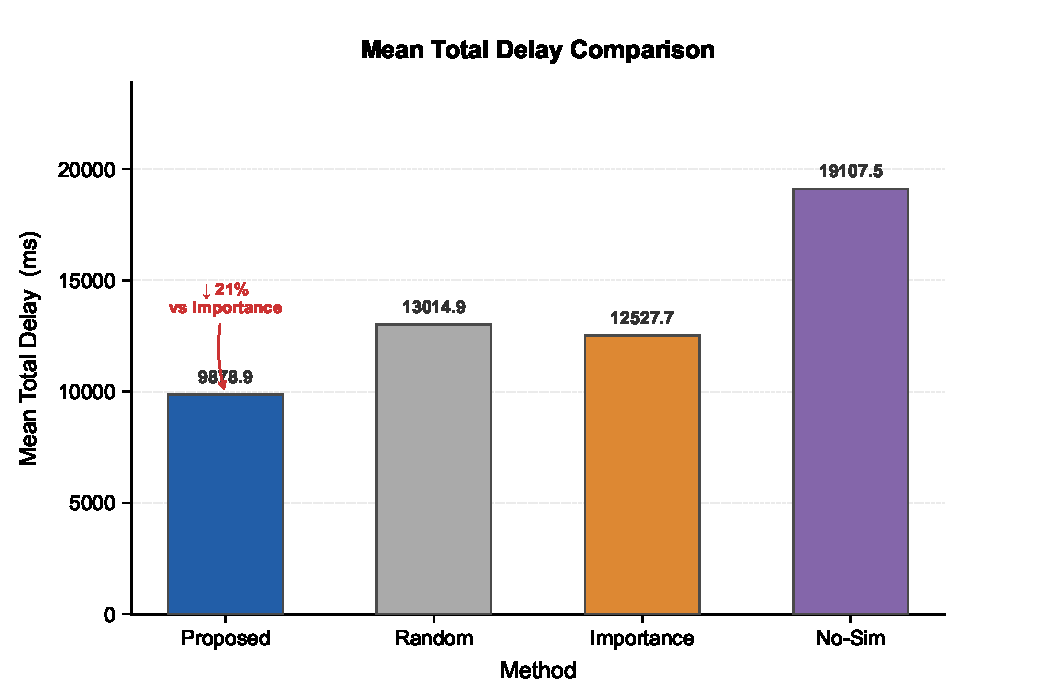
\includegraphics[width=0.92\columnwidth]{photo/fig1_total_delay.pdf}
  \caption{不同专家部署方法的平均端到端延迟对比。}
  \label{fig:total_delay}
\end{figure}

该结果表明，SimAeroMoE 的收益并非来自单一因素，而是来自需求驱动候选构造、
通信感知部署评分和动态冗余贪心选择的共同作用。Random Placement 缺乏
需求和拓扑信息，专家部署位置具有较强偶然性；Importance 虽然考虑专家需求
和部分算力因素，但仍可能把高需求专家集中到通信位置并不理想的 UAV 上；
No-Sim 则失去了相似专家带来的候选扩展和内存节省能力。因此，Proposed
能够在有限内存下同时改善专家覆盖、通信距离和计算匹配。

\subsection{Delay Breakdown}
\label{sec:delay_breakdown}

Fig.~\ref{fig:delay_breakdown} 展示了端到端延迟的组成。各方法的接入
延迟和回传延迟差异较小，因为它们共享相同的任务接入规则和无线链路模型；
主要差异来自专家计算延迟和 UAV-UAV 中间特征传输延迟。Proposed 的平均
计算延迟为 $171.8$\,ms，低于 Random Placement 的 $233.8$\,ms、
Importance 的 $231.1$\,ms 和 No-Sim 的 $394.8$\,ms；平均传输延迟为
$40.2$\,ms，也低于 Random Placement 的 $56.5$\,ms、Importance 的
$47.1$\,ms 和 No-Sim 的 $48.0$\,ms。

\begin{figure}[!t]
  \centering
  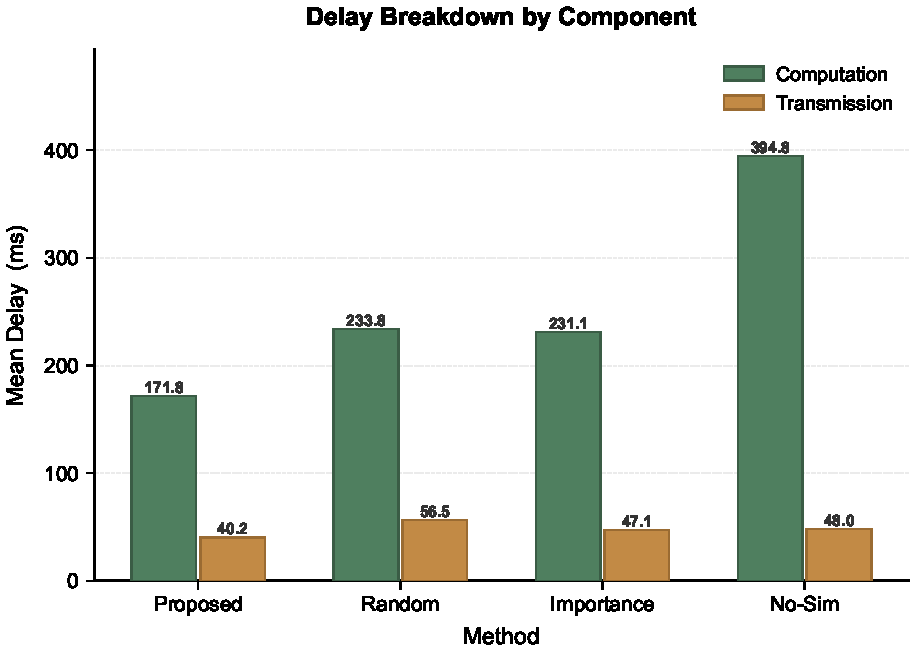
\includegraphics[width=0.92\columnwidth]{photo/fig2_delay_breakdown.pdf}
  \caption{端到端延迟分解。SimAeroMoE 通过通信感知部署和逐层调度同时降低计算与传输开销。}
  \label{fig:delay_breakdown}
\end{figure}

该分解结果与第~\ref{sec:placement_scoring}~节的评分设计一致。
$A(e,u)$ 倾向于将专家部署到能够服务本地和单跳邻域需求的位置，
从而降低跨 UAV 传输；$B(e,u)$ 倾向于将计算量较大的专家部署到算力
较强的 UAV 上；动态冗余惩罚进一步避免在同一区域重复部署功能高度重叠
的专家，使有限内存被用于更有增益的候选。No-Sim 的计算延迟最高，
主要是因为它无法使用轻量级相似专家替代原始专家，只能执行更重的精确专家。

\subsection{Similarity Substitution Analysis}
\label{sec:substitution_analysis}

Fig.~\ref{fig:substitutions} 统计了不同方法中替代专家的使用次数。
Proposed 平均产生 $114.8$ 次替代执行，高于 Random Placement 的
$85.8$ 次和 Importance 的 $89.6$ 次；No-Sim 的替代次数为 $0$。
这说明 SimAeroMoE 不仅在部署阶段把相似专家作为候选，也在在线推理调度
阶段实际利用这些替代专家来降低传输和计算代价。

\begin{figure}[!t]
  \centering
  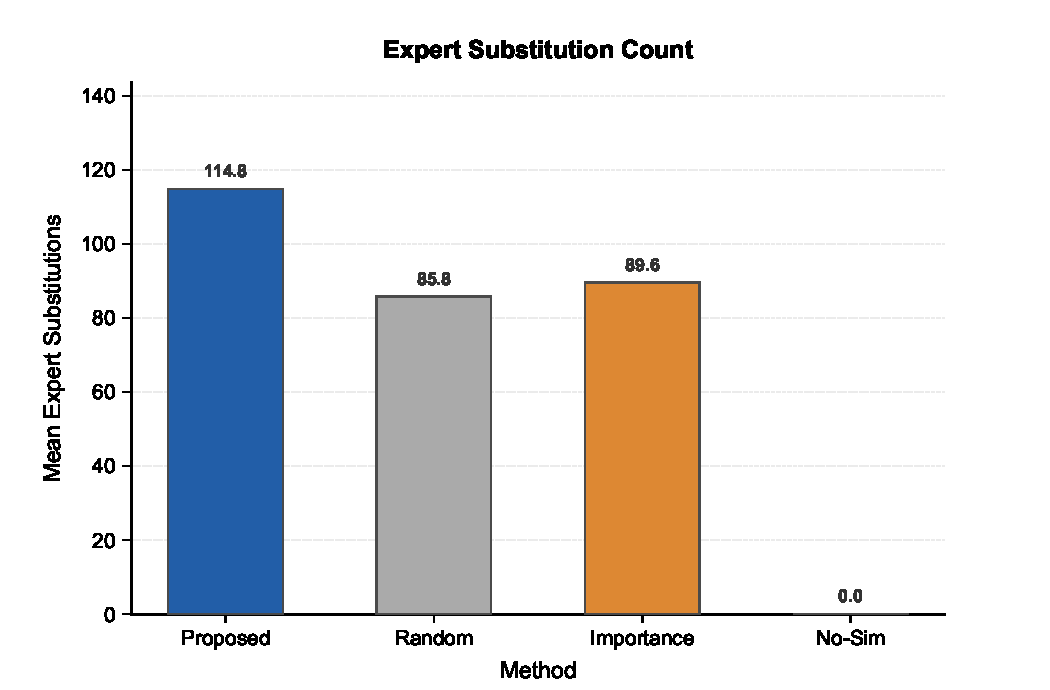
\includegraphics[width=0.92\columnwidth]{photo/fig3_substitutions.pdf}
  \caption{相似专家替代次数。Proposed 更充分地利用相似专家覆盖原始专家需求。}
  \label{fig:substitutions}
\end{figure}

相似替代机制的作用可以从两个层面解释。首先，在部署阶段，
$\mathcal{A}(r)$ 将原始需求专家扩展为可替代候选，$\mathrm{Demand}^{\mathrm{eff}}$
使替代专家继承原始专家的部分需求，从而在内存受限时提供更大的部署
选择空间。其次，在调度阶段，式~(\ref{eq:cost}) 中的误差项
$\lambda(1-\mathrm{Sim})$ 防止系统无约束地选择低质量替代专家，使延迟收益
和替代误差之间保持可控折中。

\subsection{Sensitivity Analysis}
\label{sec:sensitivity}

Fig.~\ref{fig:sensitivity_xi} 展示了相似度阈值 $\xi$ 对系统性能的影响。
当 $\xi$ 较低时，候选集合包含更多替代专家，系统具有更大的部署灵活性；
当 $\xi$ 提高时，低相似度替代被过滤，候选空间收缩。值得注意的是，
较低阈值并不意味着系统一定会选择低质量替代专家。阈值只决定候选集合，
真正执行时仍受到式~(\ref{eq:cost}) 中替代误差惩罚和累计误差约束的限制。
因此，低阈值扩大了可选空间，但不会无约束地放大多层替代偏差。

\begin{figure}[!t]
  \centering
  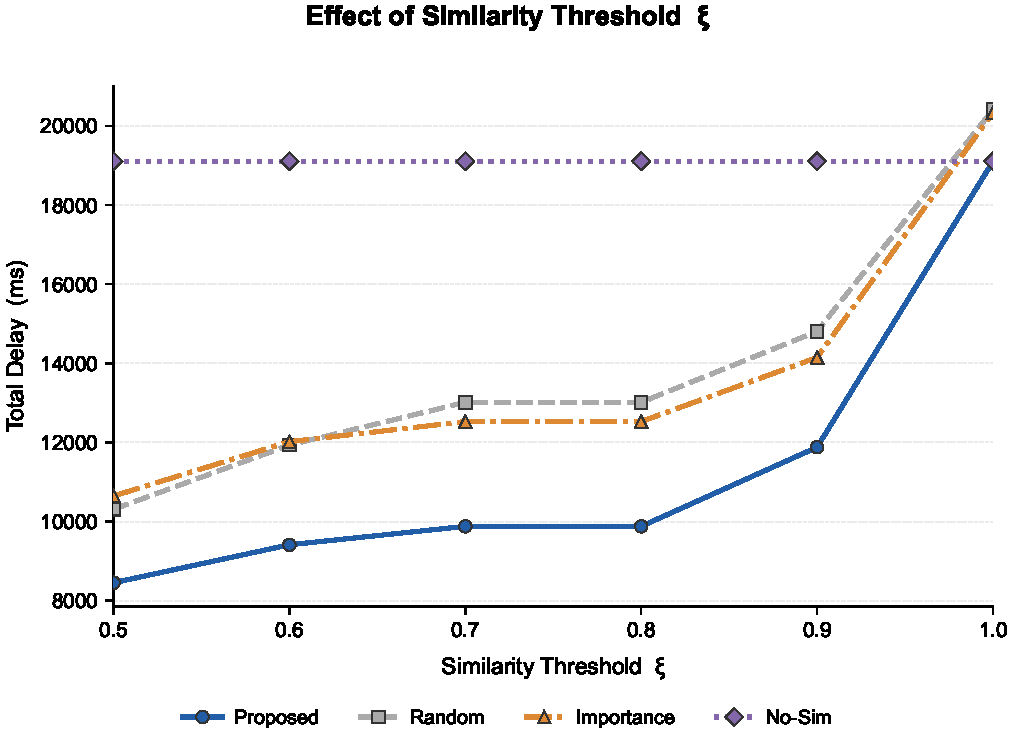
\includegraphics[width=0.92\columnwidth]{photo/fig4_sensitivity_xi.pdf}
  \caption{相似度阈值 $\xi$ 的敏感性分析。}
  \label{fig:sensitivity_xi}
\end{figure}

当 $\xi=1$ 时，只有与原始专家完全相同的专家能够进入候选集合，相似替代
事实上被关闭。此时 Proposed 退化为精确匹配策略，因此与 No-Sim 的延迟
基本重合。Random 和 Importance 在该点仍可能高于 No-Sim，这是因为它们的
部署策略分别依赖随机放置或需求排序，不能像 Proposed/No-Sim 的主流程那样
联合利用覆盖预部署和通信感知评分来优化精确专家的位置。

Fig.~\ref{fig:sensitivity_mid} 进一步分析中间特征大小的影响。随着
$S^{\mathrm{mid}}$ 增大，跨 UAV 传输开销在端到端延迟中占比上升，
通信感知部署的重要性随之增强。SimAeroMoE 通过在部署评分中显式考虑
单跳可达性和链路速率，使高需求专家更倾向于部署在可达性较好的 UAV 上。
因此，即使中间特征传输代价增大，Proposed 仍能保持较低延迟；相反，
Random 和 Importance 一旦把关键专家放在较远或链路较差的 UAV 上，
中间特征放大后会更明显地暴露通信代价。

\begin{figure}[!t]
  \centering
  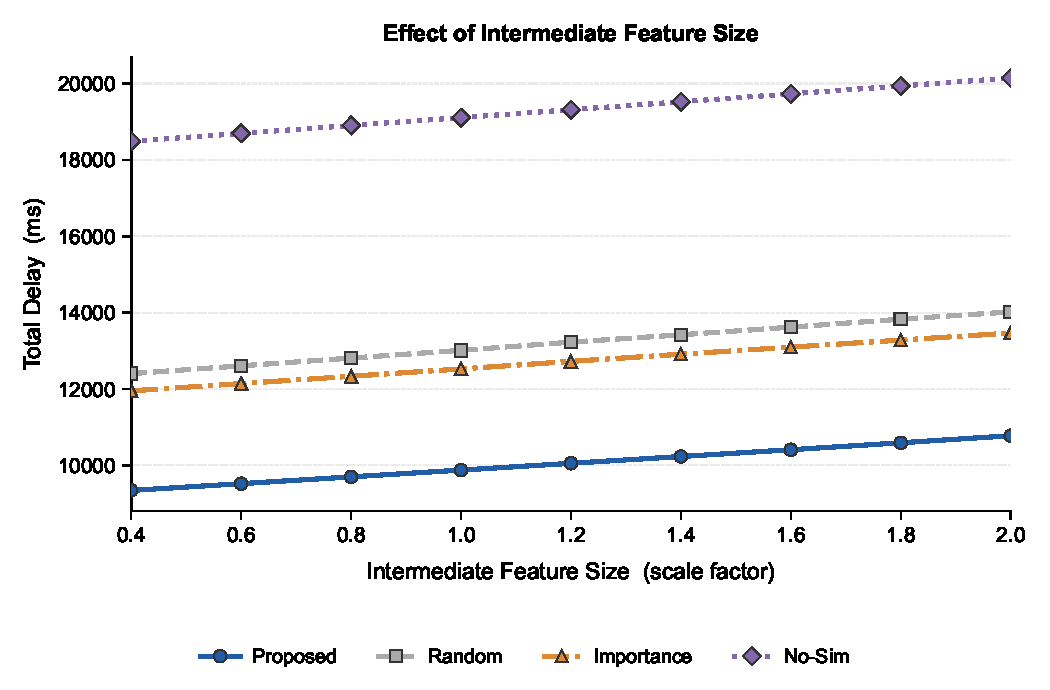
\includegraphics[width=0.92\columnwidth]{photo/fig5_sensitivity_mid_size.pdf}
  \caption{中间特征大小对端到端延迟的影响。}
  \label{fig:sensitivity_mid}
\end{figure}

Fig.~\ref{fig:sensitivity_memory} 给出了 UAV 内存容量变化时的性能趋势。
当内存较紧时，部分方法会因为无法在严格单跳调度下覆盖所有任务层而不可行。
例如，在 $0.8$ 的临界容量点，Proposed 在多数随机种子下已经可行，但其中
一个随机场景的逐层执行路径仍存在局部覆盖缺口，因此平均结果被标记为不可行。
这说明部署阶段的覆盖预部署是面向专家需求和局部连通性的近似保证，真正的
可行性还需要在执行阶段逐层检查当前 UAV 到下一专家位置的单跳可达性和替代误差。

\begin{figure}[!t]
  \centering
  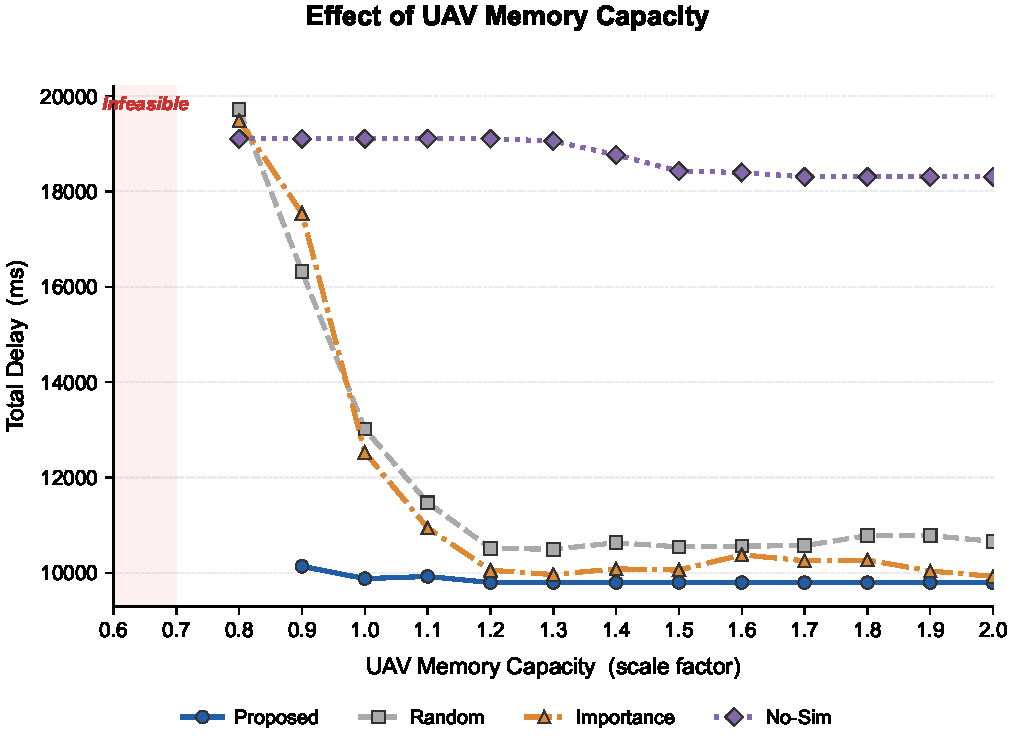
\includegraphics[width=0.92\columnwidth]{photo/fig6_sensitivity_memory.pdf}
  \caption{UAV 内存容量对端到端延迟和部署规模的影响。}
  \label{fig:sensitivity_memory}
\end{figure}

随着内存容量增加，各方法能够部署更多专家，因此 Random 和 Importance 的
延迟逐渐下降并接近 Proposed。这种接近主要来自关键专家被逐步放入 UAV 内存后，
通信路径和专家覆盖得到改善；但该趋势并不意味着基线获得了相同的部署能力。
在 $1.5$ 的容量比例下，Random 和 Importance 仍分别比 Proposed 高约
$7.6\%$ 和 $2.7\%$，而 No-Sim 仍高约 $88.1\%$。图中后段差距看起来较小，
部分原因是 No-Sim 的高延迟拉大了纵轴范围，压缩了其他三条曲线之间的视觉差异。

\subsection{Scalability Analysis}
\label{sec:scalability}

除上述参数敏感性外，本文进一步考察系统规模变化时的性能。Fig.~\ref{fig:scale_uav}
仅增加 UAV 数量，并保持任务和专家设置不变。随着 UAV 数量从 4 增加到
20，Proposed 的平均单任务延迟从 $175.2$\,ms 降至 $161.9$\,ms，并始终
低于所有基线。Proposed 曲线相对平稳，是因为在 UAV 较少时它已经通过相似
替代和通信感知部署较充分地利用了有限资源；当 UAV 继续增加时，额外位置
带来的边际收益相对有限。

\begin{figure}[!t]
  \centering
  \IfFileExists{photo/fig7_uav_count.pdf}{%
    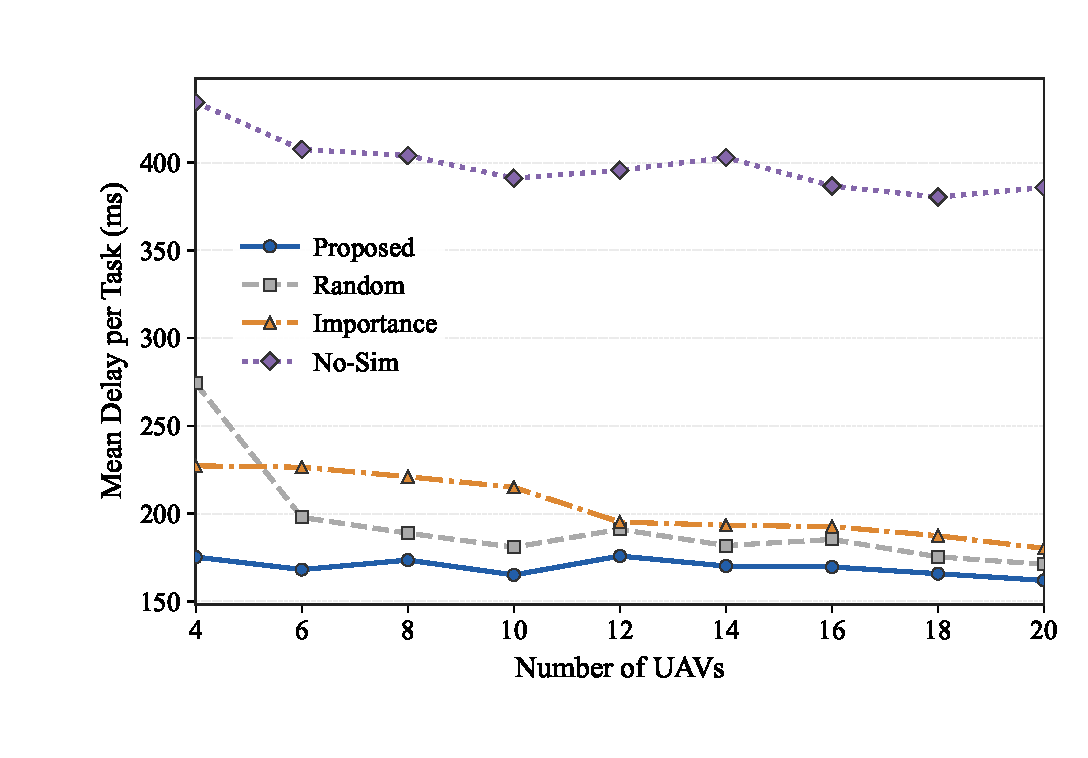
\includegraphics[width=0.92\columnwidth]{photo/fig7_uav_count.pdf}%
  }{%
    \fbox{\parbox{0.88\columnwidth}{\centering Missing figure file:\\
    photo/fig7\_uav\_count.pdf}}%
  }
  \caption{UAV 数量变化下的扩展性。}
  \label{fig:scale_uav}
\end{figure}

相比之下，Random 和 Importance 随 UAV 数量增加改善更明显。Random 虽然
缺乏策略，但 UAV 数量变多后，随机部署碰巧覆盖任务附近区域的概率提高；
Importance 则能够把更多高需求专家放入系统，但由于它不显式优化逐层通信路径，
在部分点上可能不如随机分散部署。No-Sim 也受益于更多 UAV 提供的存储和位置，
但由于不能用相似专家合并需求，其延迟仍显著高于其他方法。

Fig.~\ref{fig:scale_task} 仅增加任务数量，并保持 UAV、专家池和区域大小不变。
当任务数从 20 增加到 100 时，各方法的平均单任务延迟整体保持稳定，说明
任务数量增加主要改变需求统计样本量和调度次数，而不会直接改变单个任务的
通信距离、可达结构和专家计算量。Proposed 在所有任务规模下保持最低延迟，
表明需求驱动的有效专家建模能够从更多任务样本中提取稳定的部署偏好。

\begin{figure}[!t]
  \centering
  \IfFileExists{photo/fig8_task_count.pdf}{%
    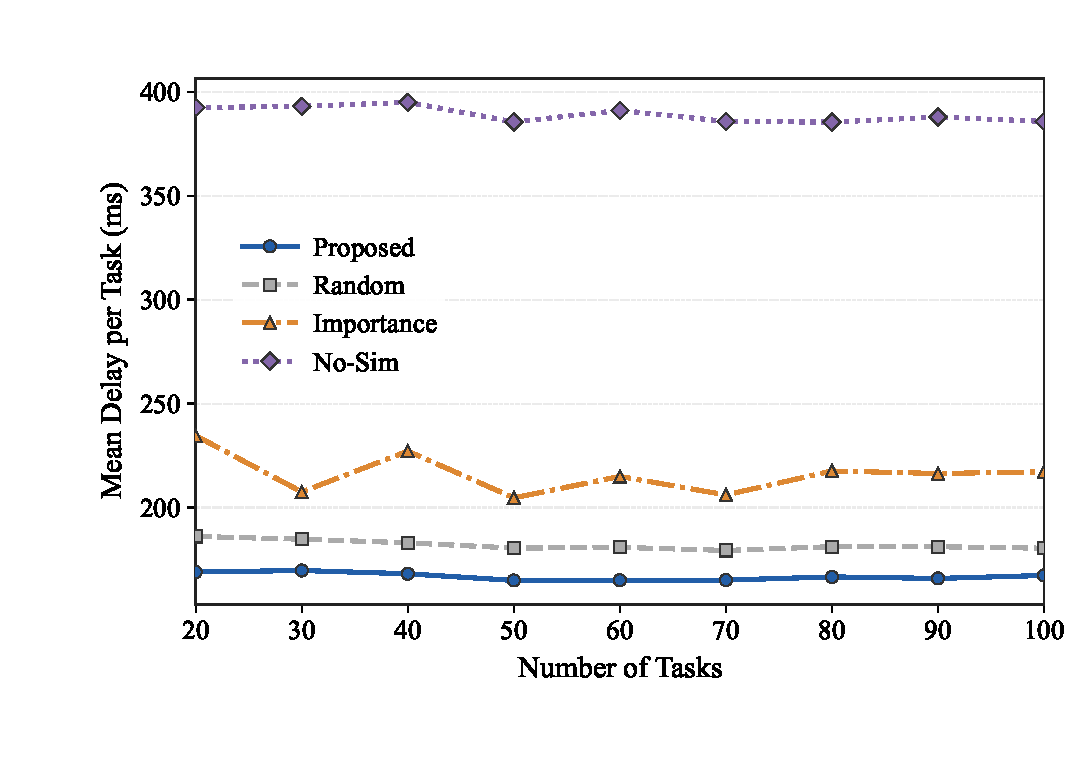
\includegraphics[width=0.92\columnwidth]{photo/fig8_task_count.pdf}%
  }{%
    \fbox{\parbox{0.88\columnwidth}{\centering Missing figure file:\\
    photo/fig8\_task\_count.pdf}}%
  }
  \caption{任务数量变化下的平均单任务延迟。}
  \label{fig:scale_task}
\end{figure}

在 Fig.~\ref{fig:scale_task} 中，Random 在若干点上低于 Importance。
这并不表示随机部署本质上更优，而是说明当前 UAV 场景中通信位置可能比全局
专家重要性更主导延迟。Importance 倾向于优先部署高需求专家并利用高算力 UAV，
但如果这些 UAV 的空间位置并不靠近主要任务入口，逐层传输代价会升高；
Random 的分散放置反而可能在某些热点场景下提供更好的空间覆盖。Proposed
通过同时考虑需求、相似性和通信可达性，避免了这两类基线各自的偏差。

Fig.~\ref{fig:scale_expert} 进一步仅增加专家池规模。专家数量增加一方面扩大
候选部署空间，另一方面也使任务需求分布到更大的专家集合上，从而加重 UAV
内存竞争。Proposed 在 8--24 个专家范围内保持最低任务延迟；在 24 个专家时，
Proposed 仍保持可行且单任务延迟为 $173.7$\,ms，而 Random 和 Importance 的
成功率均降至 $0.2$，No-Sim 则完全不可行。

\begin{figure}[!t]
  \centering
  \IfFileExists{photo/fig9_expert_count.pdf}{%
    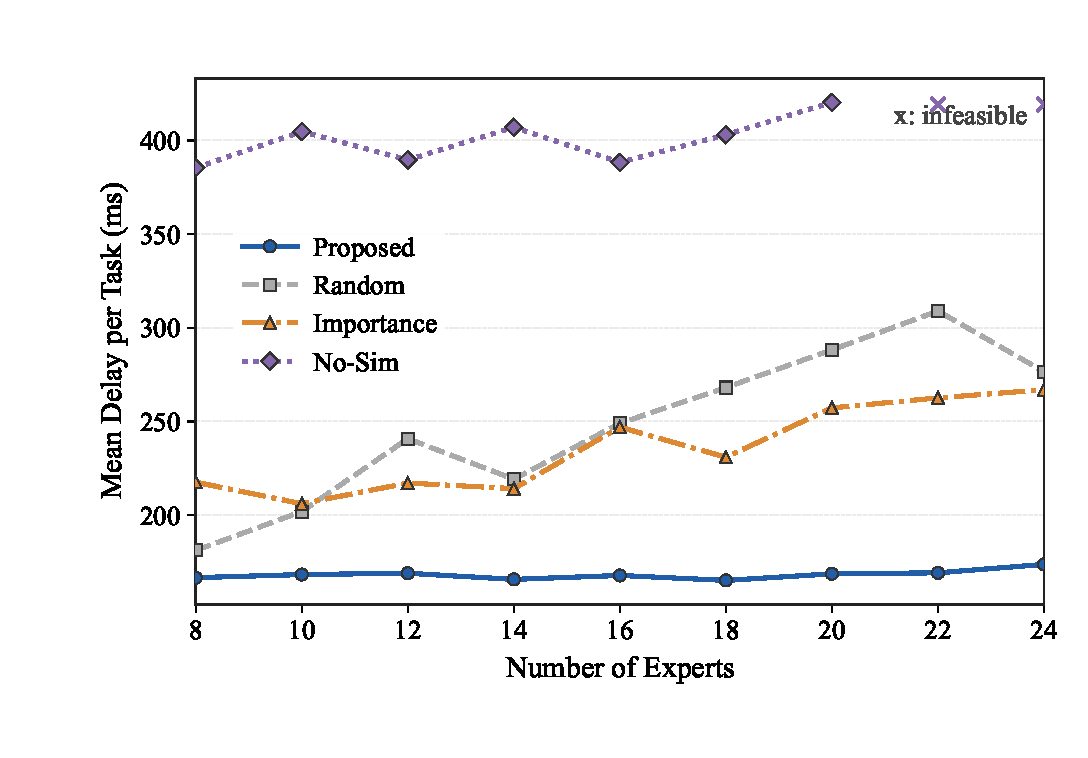
\includegraphics[width=0.92\columnwidth]{photo/fig9_expert_count.pdf}%
  }{%
    \fbox{\parbox{0.88\columnwidth}{\centering Missing figure file:\\
    photo/fig9\_expert\_count.pdf}}%
  }
  \caption{专家池规模变化下的扩展性。}
  \label{fig:scale_expert}
\end{figure}

该现象体现了相似替代在专家空间扩大时的价值。新增专家并不只是增加候选数量，
也会让任务请求更加分散。No-Sim 必须精确部署每个被请求的原始专家，因此在
固定 UAV 内存下更容易出现覆盖缺口；Random 和 Importance 虽然可以部署替代
候选，但缺乏通信感知和冗余控制，专家池变大后更容易把容量消耗在低收益位置。
Proposed 则通过相似候选构造把多个相近需求合并到较少的部署专家上，并通过
动态冗余惩罚避免功能重复部署，因此在专家池扩大时仍能保持较好的可行性和延迟。

Fig.~\ref{fig:scale_area} 分析部署区域扩大时的影响。该实验包含两种设置：
一是固定 UAV、任务和专家资源，仅扩大区域边长；二是随区域扩大同步增加
系统资源。在固定资源设置下，区域从 $250\,\mathrm{m}\times250\,\mathrm{m}$
扩大到 $1000\,\mathrm{m}\times1000\,\mathrm{m}$ 后，单跳可达性快速下降，
部分基线在大区域下出现不可行。Proposed 仍能在更大范围内保持较高成功率，
但成功率也会随区域扩大而下降。这一结果并不与本文目标矛盾：本文主要研究
单跳 UAV 协同推理，适用于覆盖范围不过大的局部空中边缘网络。当部署范围
过大时，中间特征传输可能超出单跳通信半径，或者为了覆盖更多远端需求而
需要在 UAV 上存放过多专家，进而触发内存不足问题。实际系统可通过多跳
转发、区域分簇或分层 UAV 中继扩展覆盖范围；这些机制会引入新的路由和
队列开销，本文将其留作后续工作。在全系统同步扩展设置下，各方法的延迟
更平稳，说明区域扩大本身并非不可处理，关键在于通信半径、UAV 数量和
内存资源需要随覆盖范围匹配扩展。

\begin{figure}[!t]
  \centering
  \IfFileExists{photo/fig10_area_scaling.pdf}{%
    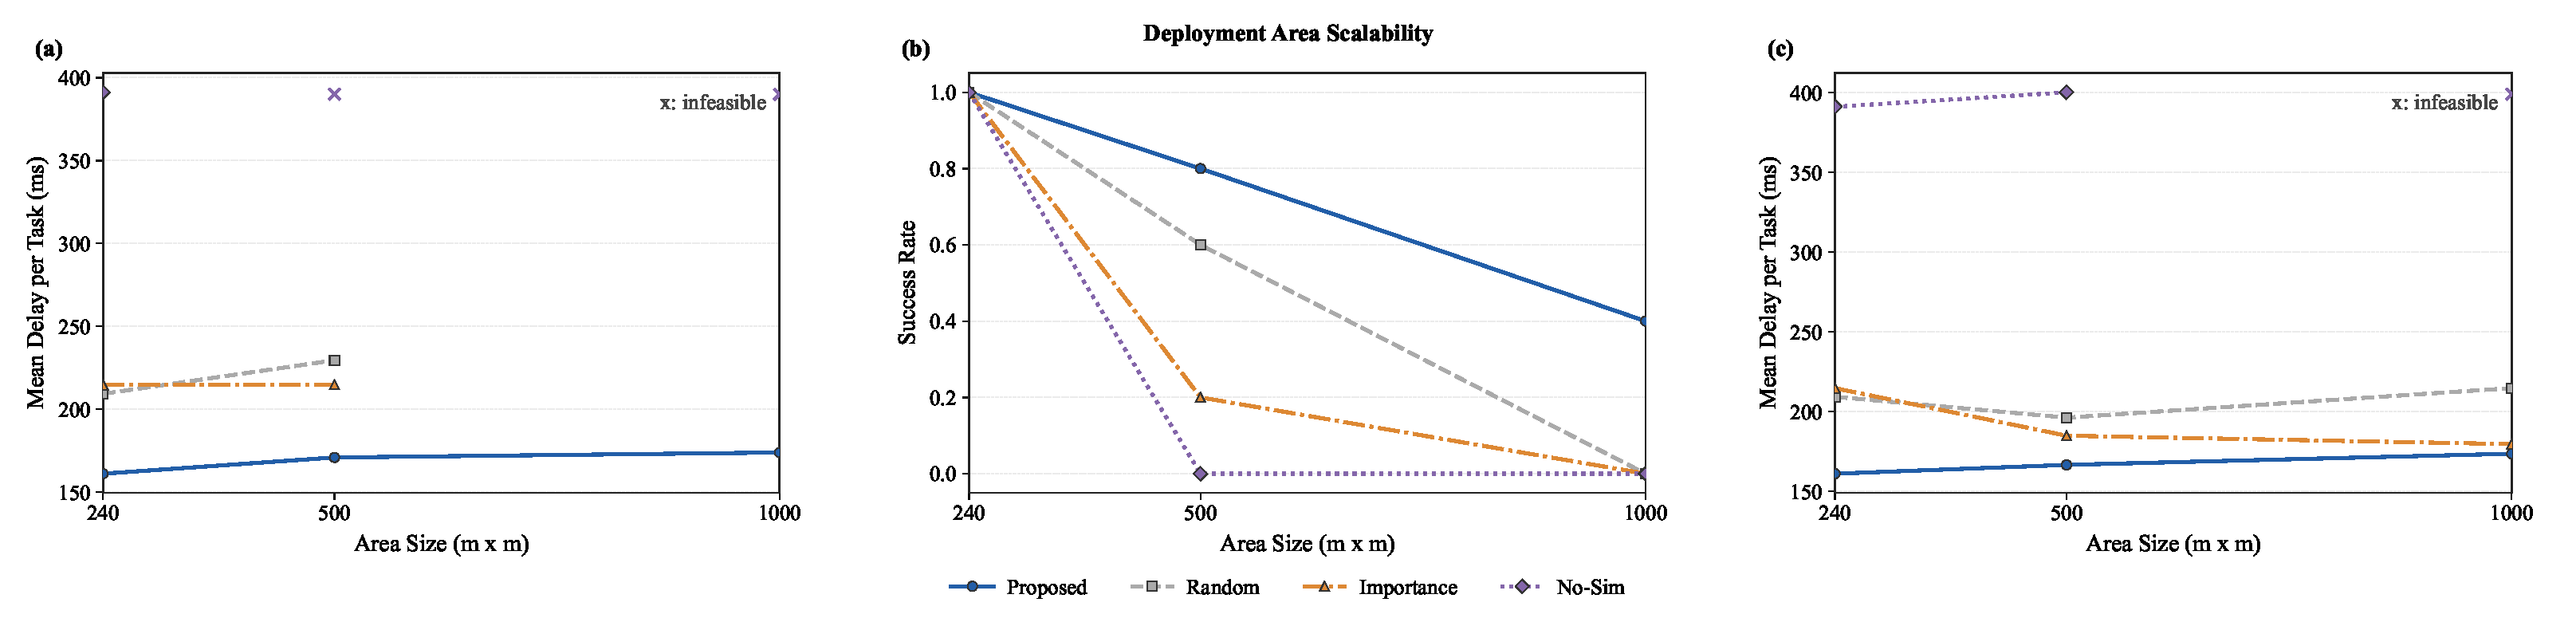
\includegraphics[width=0.92\columnwidth]{photo/fig10_area_scaling.pdf}%
  }{%
    \fbox{\parbox{0.88\columnwidth}{\centering Missing figure file:\\
    photo/fig10\_area\_scaling.pdf}}%
  }
  \caption{部署区域大小变化下的扩展性。固定资源时，大范围场景会因单跳连通性和 UAV 内存限制而降低可行性；同步扩展资源后可维持稳定服务。}
  \label{fig:scale_area}
\end{figure}

Fig.~\ref{fig:advantage_scenario} 进一步给出了本文方法的优势场景。该实验固定
10 架 UAV 和 80 个任务，将专家池设为 20 类，并逐步压缩 UAV 的专家存储容量，
从而形成“任务需求异构、专家类型较多、单个 UAV 内存受限”的压力场景。
当内存比例较低时，Random 和 Importance 容易把有限存储分配给与当前任务或位置
不匹配的专家，No-Sim 又必须精确部署原始专家，因此可行性明显下降。相比之下，
Proposed 可以利用相似专家替代把多个相近需求合并到较少的部署专家上，同时通过
通信感知评分选择更合适的 UAV 位置，因此在紧内存区间仍能保持较高成功率和较低
单任务延迟。随着内存逐渐放宽，基线方法的可行性和延迟会改善，但 Proposed 仍保持
稳定优势，说明本文方法的收益主要来自资源受限条件下的替代弹性和部署匹配，而不是
单纯依赖更多存储空间。

\begin{figure}[!t]
  \centering
  \IfFileExists{photo/fig11_advantage_scenario.pdf}{%
    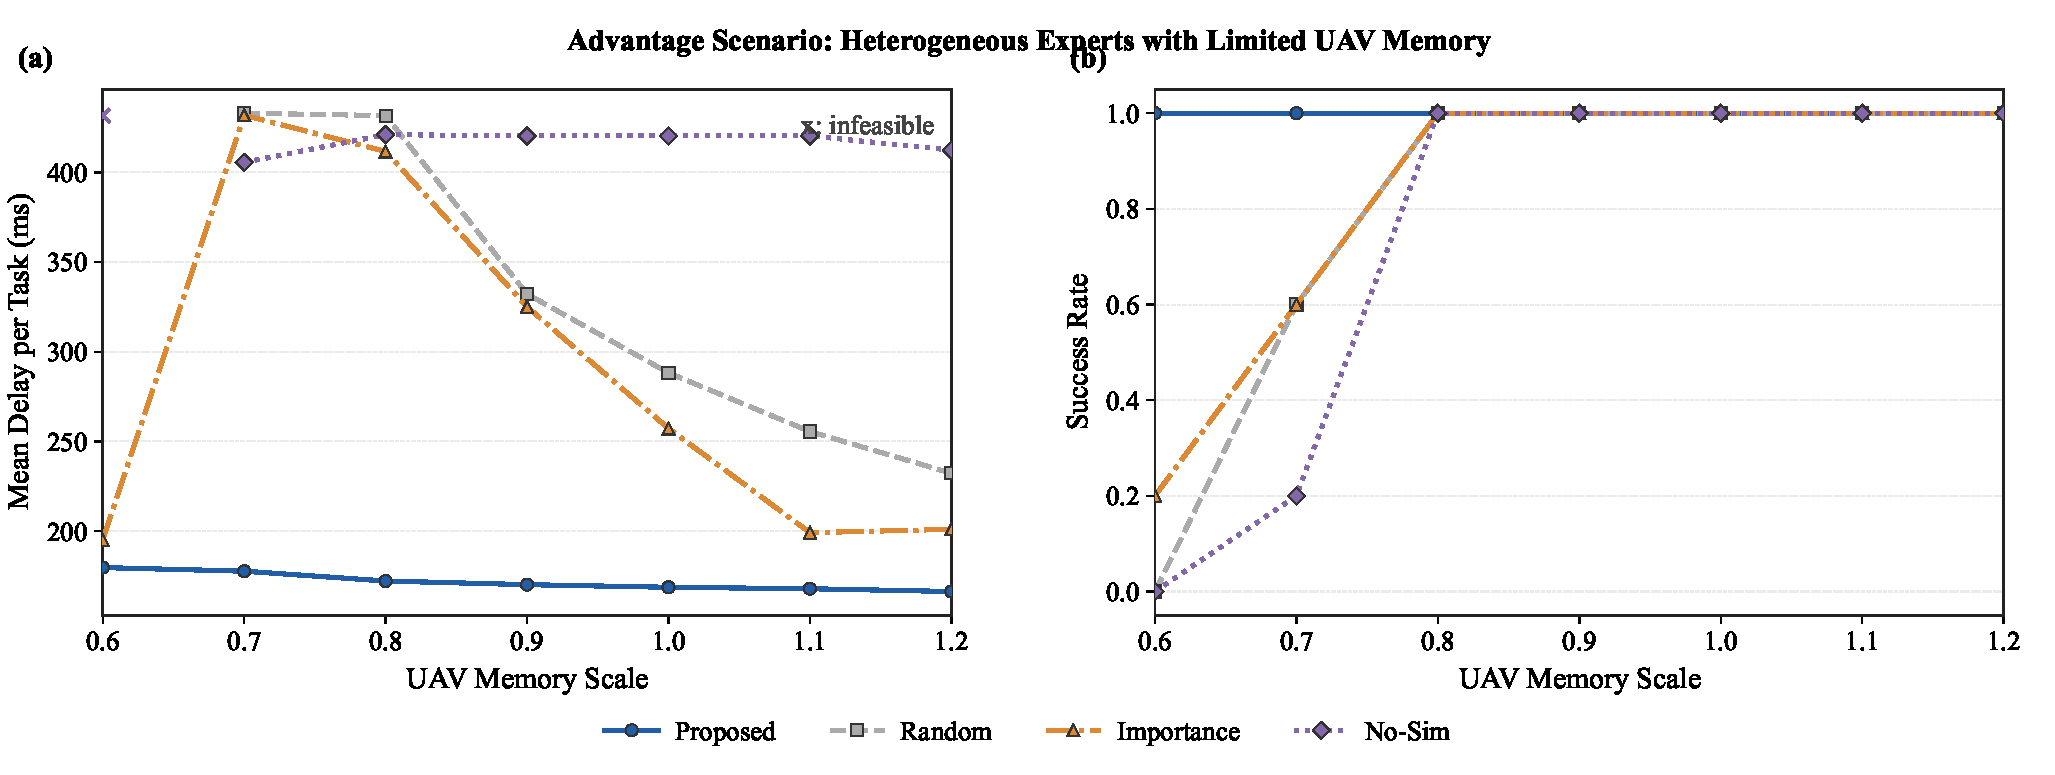
\includegraphics[width=0.92\columnwidth]{photo/fig11_advantage_scenario.pdf}%
  }{%
    \fbox{\parbox{0.88\columnwidth}{\centering Missing figure file:\\
    photo/fig11\_advantage\_scenario.pdf}}%
  }
  \caption{资源受限异构专家需求下的优势场景。该图固定任务规模和专家池规模，仅改变 UAV 专家存储容量，以展示相似替代和通信感知部署在紧内存场景中的可行性与延迟优势。}
  \label{fig:advantage_scenario}
\end{figure}

总体来看，仿真实验验证了第~\ref{sec:design}~节的核心设计：相似候选
构造扩展了可部署专家空间，通信感知评分改善了专家与 UAV 的匹配，动态
冗余贪心在内存约束下避免功能重复部署，而轻量级逐层调度将部署结果转化
为更低的端到端推理延迟。扩展性实验进一步说明，SimAeroMoE 在 UAV、
任务和专家规模增加时能够保持稳定优势；对于超出单跳覆盖假设的大范围场景，
其主要限制来自连通性和 UAV 内存容量，需要结合多跳或分簇机制进一步扩展。

% ==============================================================
\section{Related Work}
\label{sec:related}
% ==============================================================

\textbf{UAV 边缘智能。}
UAV 网络能够通过灵活部署、视距通信和按需覆盖为地面任务提供空中边缘服务，
因此被广泛用于无线覆盖、应急通信、搜索救援和边缘计算等场景
~\cite{mozaffari2019uav,zhu2019uav}。现有 UAV 边缘计算研究通常关注
轨迹规划、任务卸载、链路资源分配和服务覆盖等问题，其核心目标是在受限
通信和能量条件下降低任务处理时延或提高系统吞吐。然而，这类工作大多将
推理任务视为整体计算负载，或者只考虑普通 DNN 模型在 UAV 或边缘节点上的
卸载执行，较少利用 MoE 模型中按需激活专家的稀疏结构。与上述工作不同，
本文将 UAV 协同推理问题细化到专家级部署和逐层专家执行调度，并在单跳
UAV-UAV 通信约束下联合考虑专家需求、内存限制和跨 UAV 传输开销。

\textbf{边缘模型部署与协同推理。}
边缘智能研究表明，将深度模型推理下沉到边缘设备可以降低云端依赖并改善
实时性~\cite{zhou2019edge}。已有协同推理系统通过模型划分、流水线执行或
异构处理器协同来提升边缘推理性能。例如，CoEdge~\cite{zeng2020coedge}
将 DNN 推理任务划分到多个异构边缘设备上执行，CoDL~\cite{jia2022codl}
关注移动设备内部 CPU-GPU 协同推理，BAND~\cite{jeong2022band} 和
Asymo~\cite{wang2021asymo} 则分别从带宽感知调度和非对称核心调度角度
优化边缘推理。上述方法主要面向普通 DNN 或设备内部异构计算，部署粒度
通常是模型层、算子或任务分片。SimAeroMoE 的部署粒度是 MoE 专家，系统
需要决定哪些专家或相似替代专家应部署在哪些 UAV 上，并进一步根据部署
结果选择每一步专家执行位置。因此，本文关注的不是一般模型划分问题，而是
内存受限 UAV 网络中的专家级缓存、替代和通信感知调度问题。

\textbf{MoE 模型服务与专家路由。}
MoE 通过稀疏激活机制在较低单次计算成本下扩展模型容量，代表性工作包括
Sparsely-Gated MoE~\cite{shazeer2017moe}、Switch Transformer
~\cite{fedus2022switch}、GShard~\cite{lepikhin2021gshard} 和
Mixtral~\cite{jiang2024mixtral}。此外，Expert-Choice routing
~\cite{zhou2022mixtureofexperts_routing} 和 GLaM~\cite{du2022glam}
从路由机制和负载均衡角度提升 MoE 模型的训练或推理效率。系统层面的
MoE 服务研究通常部署在云端或数据中心环境中，例如 DeepSpeed-Inference
~\cite{aminabadi2022deepspeed}、Orca~\cite{yu2022orca} 和
AlpaServe~\cite{li2023alpaserve} 等工作主要面向资源相对充足、网络较为
稳定的服务器集群，重点优化吞吐、批处理、并行执行和负载均衡。相比之下，
UAV 边缘环境具有内存容量小、设备异构、链路带宽受限和连通关系动态变化等
特点，不能直接采用面向数据中心的专家并行和全量专家部署策略。

\textbf{本文区别。}
综上，已有研究分别从 UAV 边缘计算、边缘协同推理和 MoE 服务优化等角度
解决了部分相关问题，但尚未充分考虑 UAV 边缘网络中 MoE 专家之间的相似
替代关系。本文提出的 SimAeroMoE 将专家相似性显式纳入候选专家构造、部署
评分和推理调度过程：首先根据任务需求和相似度阈值构造可替代专家集合，
然后通过覆盖预部署保证原始专家需求可服务，再利用动态贪心算法在剩余内存
下选择具有较高通信和计算收益的专家部署位置。该设计使系统能够在不部署
所有原始专家的情况下，通过相似性约束的替代机制缓解 UAV 内存压力，并在
单跳通信约束下降低端到端推理延迟。

% ==============================================================
\section{Conclusion}
\label{sec:conclusion}
% ==============================================================

本文研究了 UAV 边缘网络中的 MoE 协同推理问题，重点关注在 UAV 内存、
计算能力和单跳通信链路受限的条件下，如何进行专家级部署与推理调度以
降低端到端延迟。针对直接部署原始专家容易造成内存压力、忽略通信拓扑又会
增加跨 UAV 传输开销的问题，本文提出 SimAeroMoE，将专家相似性、任务需求、
UAV 资源约束和通信关系共同纳入部署决策。

SimAeroMoE 首先根据任务分布统计各 UAV 区域的专家需求，并基于专家相似度
构造可替代专家集合；随后设计通信感知的专家部署评分，并采用两阶段动态
贪心策略完成专家部署，其中预部署阶段保证必要专家需求可服务，动态调整
阶段在剩余内存中选择收益更高、冗余更低的专家部署方案。最后，SimAeroMoE
根据部署结果执行轻量级逐层调度，为每个专家执行步骤选择本地或单跳可达的
UAV。

仿真实验结果表明，在本文设置的随机热点 UAV 场景中，SimAeroMoE 相比
Random Placement、Importance 和 No-Sim
分别降低了约 $24.1\%$、$21.3\%$ 和 $48.2\%$ 的平均端到端推理延迟。
结果说明，相似专家替代能够缓解内存受限下的专家覆盖压力，通信感知部署
能够减少不必要的跨 UAV 传输，从而提升 UAV 边缘 MoE 协同推理效率。

% ---- references ----------------------------------------------
\bibliographystyle{IEEEtran}
\bibliography{IEEEabrv,refs}

\end{CJK*}
\end{document}
